\chapter{Flavour Tagging}
\textit{This Appendix lists some additional results in support of Chapter \ref{chap-ftag}.}

\section{DL1d with Variable Radius Jets}\label{ap-DL1dVR}
This section presents some plots on the VR-training of DL1d. Figure \ref{apfig:DL1dVRscanf} displays some flavour fractions scans for the $b$-tagging and $c$-tagging. 

\begin{figure}[h!]
  \centering
  \begin{subfigure}[b]{\textwidth}
      \centering
      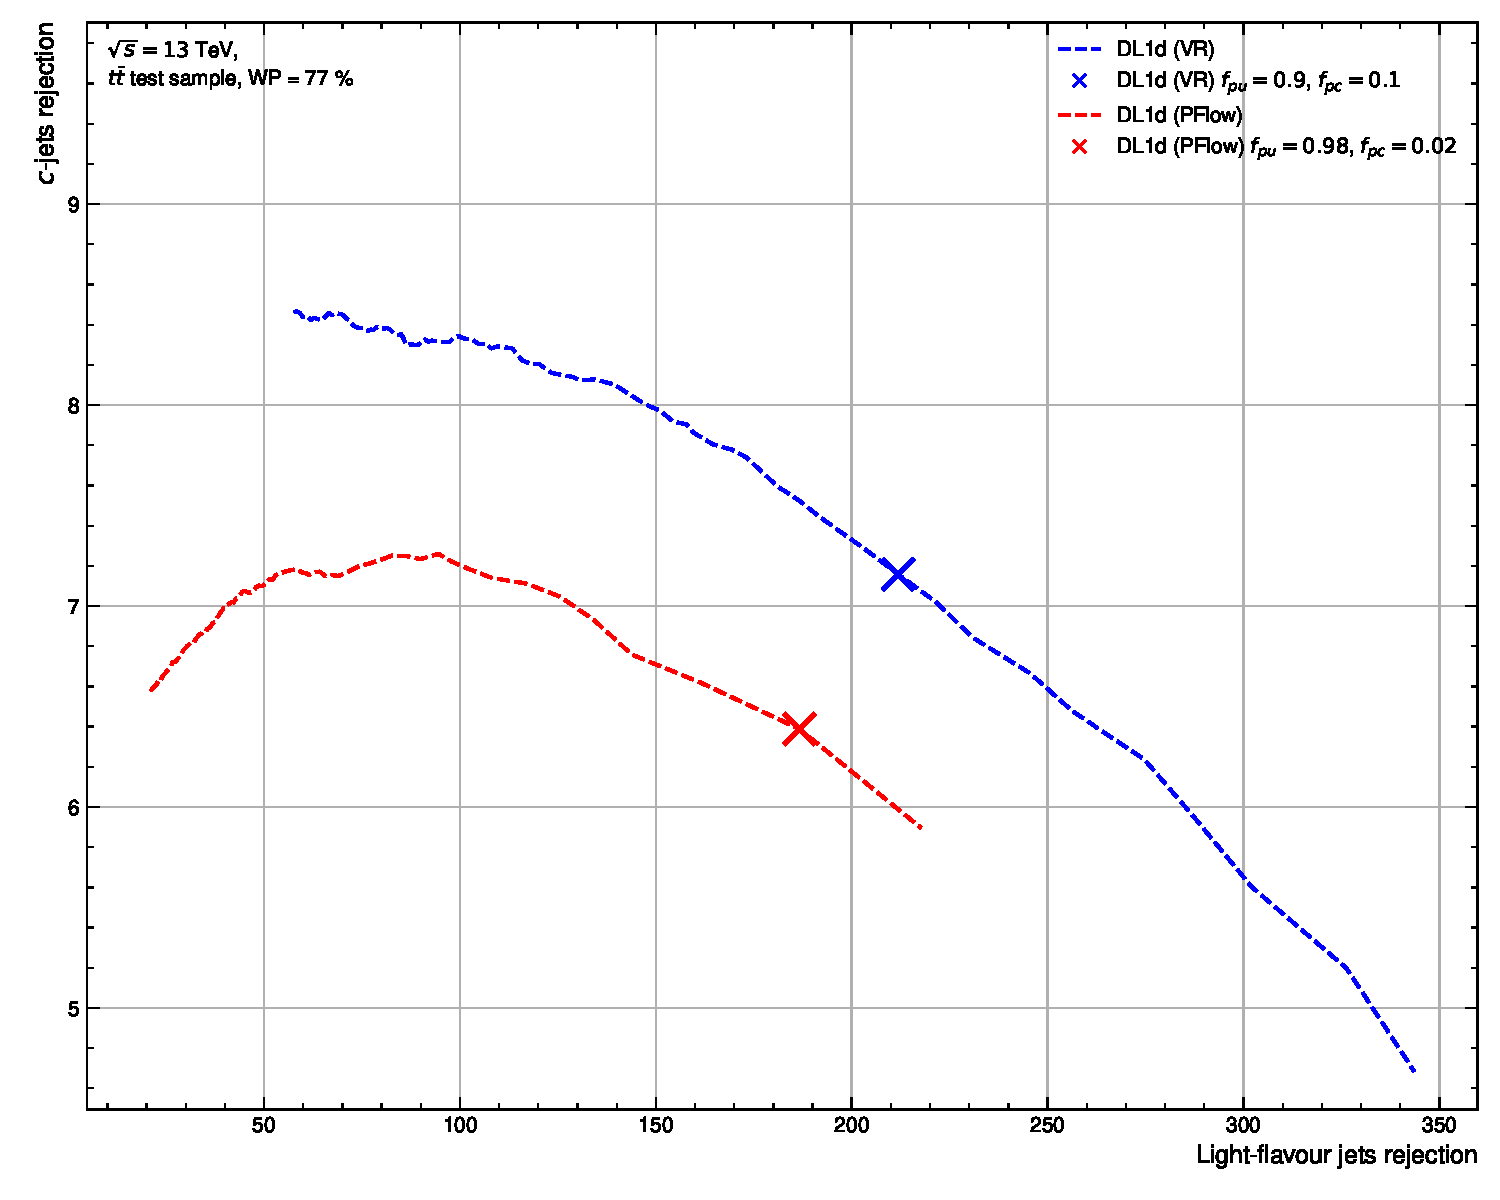
\includegraphics[width=0.32\textwidth]{Images/FTAG/VRDL1d/scansfraction/thesis_plot_frac/contour_fraction_ttbar_200.pdf}
      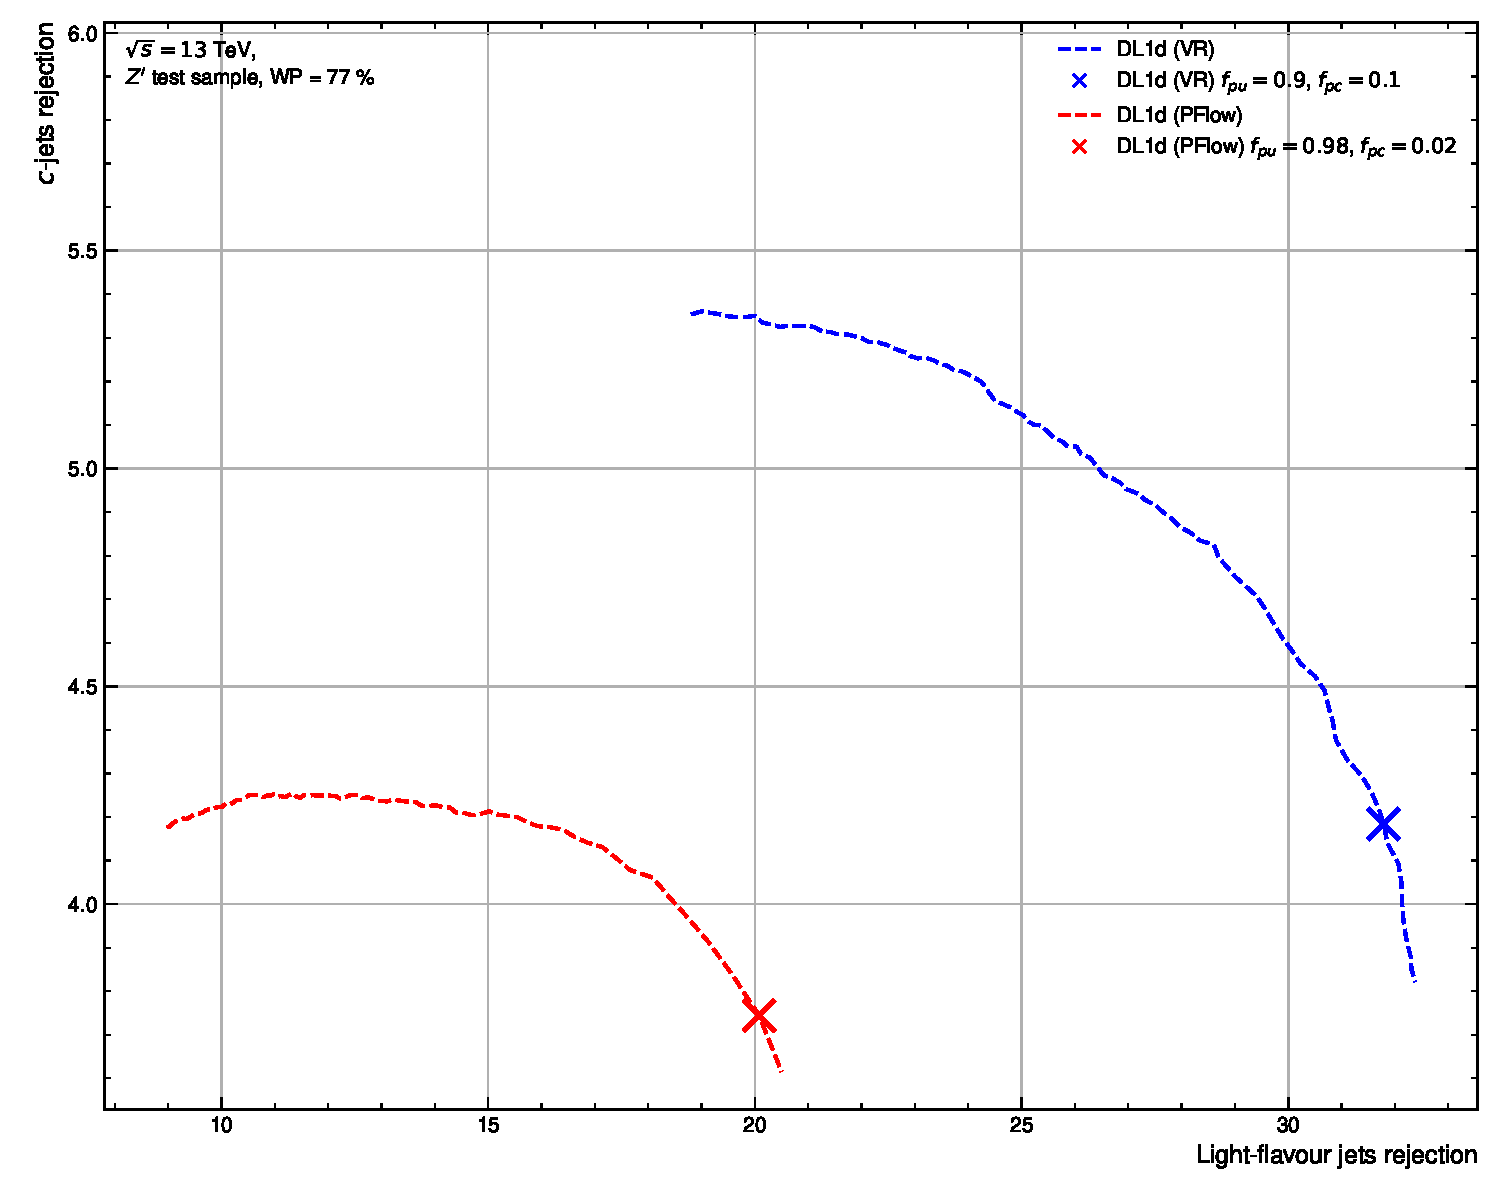
\includegraphics[width=0.32\textwidth]{Images/FTAG/VRDL1d/scansfraction/thesis_plot_frac/contour_fraction_zpext_200.pdf}
      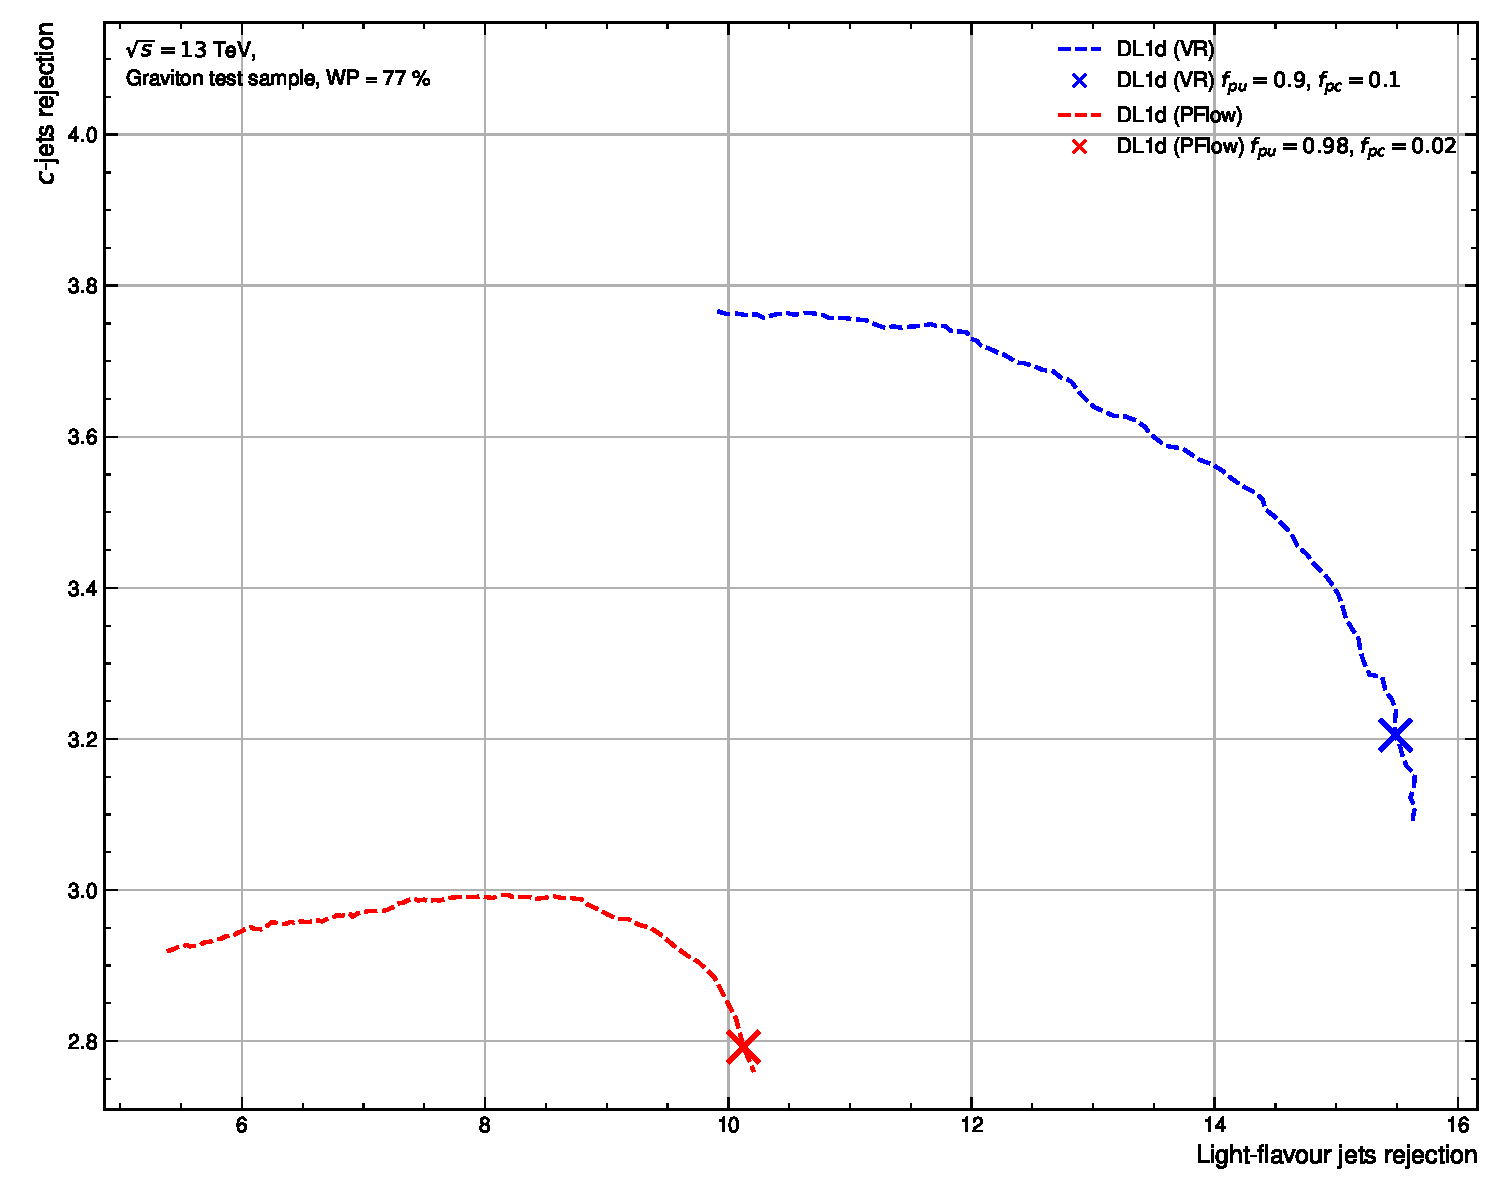
\includegraphics[width=0.32\textwidth]{Images/FTAG/VRDL1d/scansfraction/thesis_plot_frac/contour_fraction_graviton_200.pdf}
      \caption{Flavour fraction $f_c^b$ for $b$-tagging scans.} 
      \label{fig:DL1dVRscanfb}
  \end{subfigure}\\
  \begin{subfigure}[b]{\textwidth}
    \centering % UNreadable: increase font size
    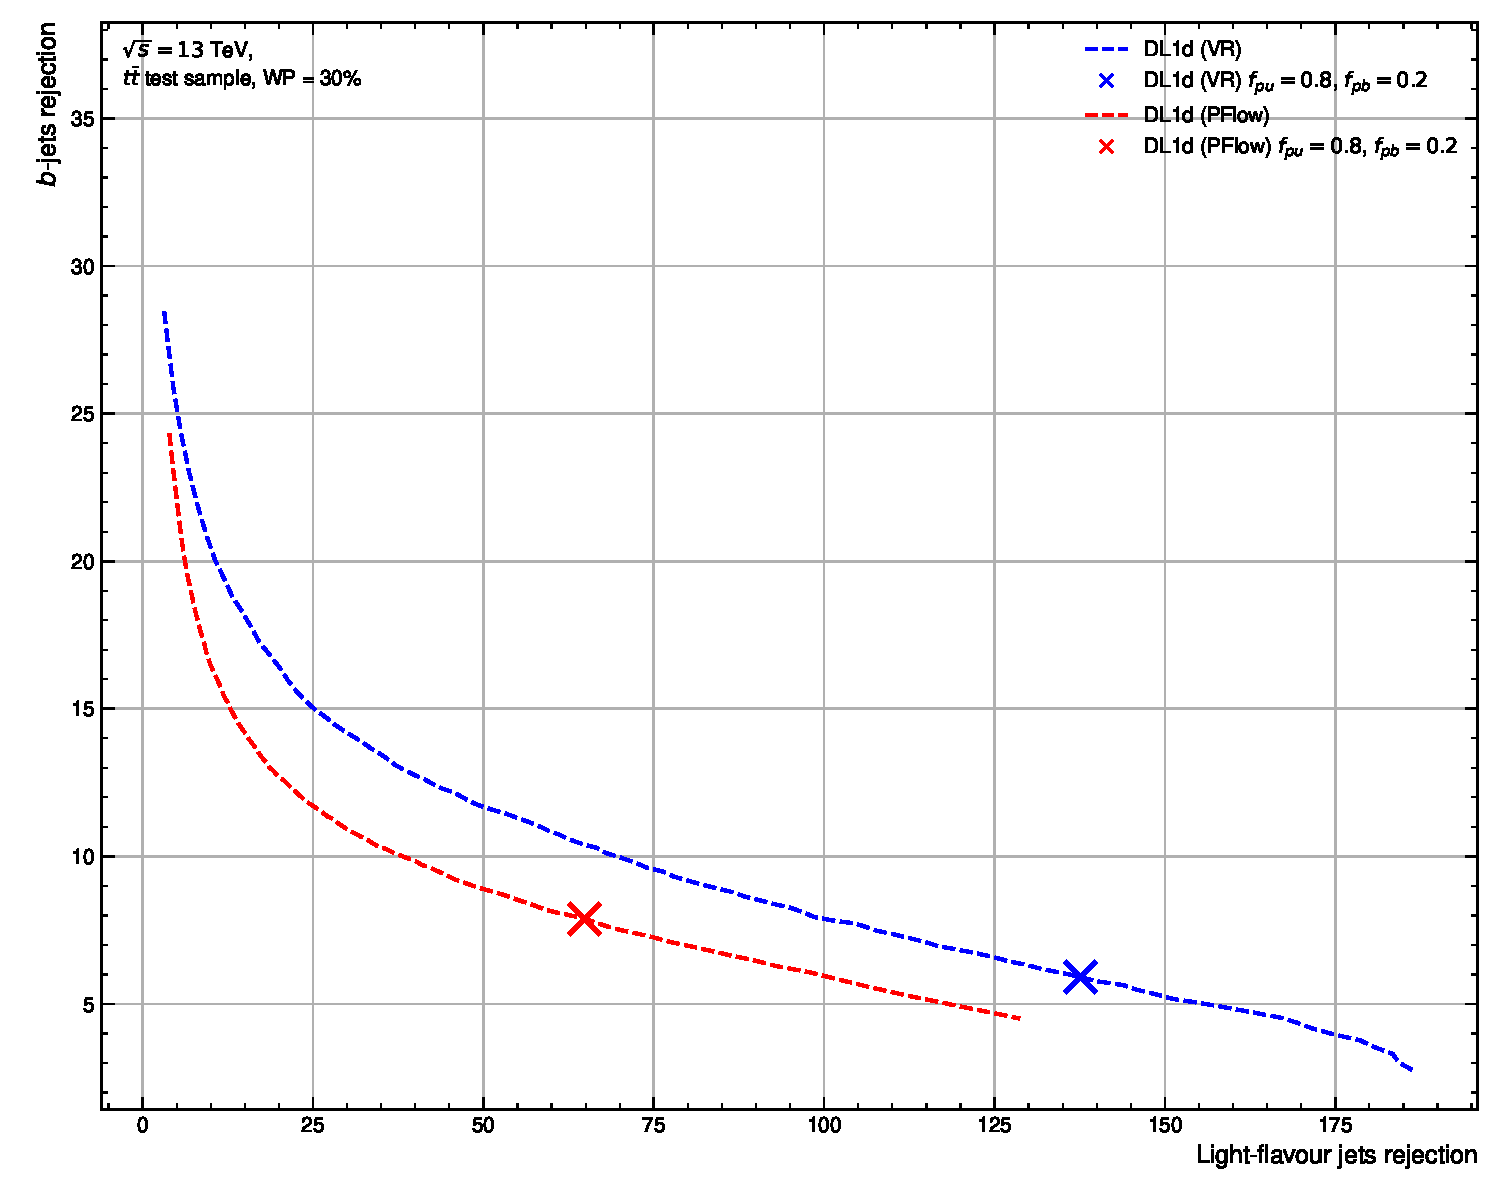
\includegraphics[width=0.32\textwidth]{Images/FTAG/VRDL1d/scansfraction/thesis_plot_frac_c/contour_fraction_ttbar_2000.pdf}
    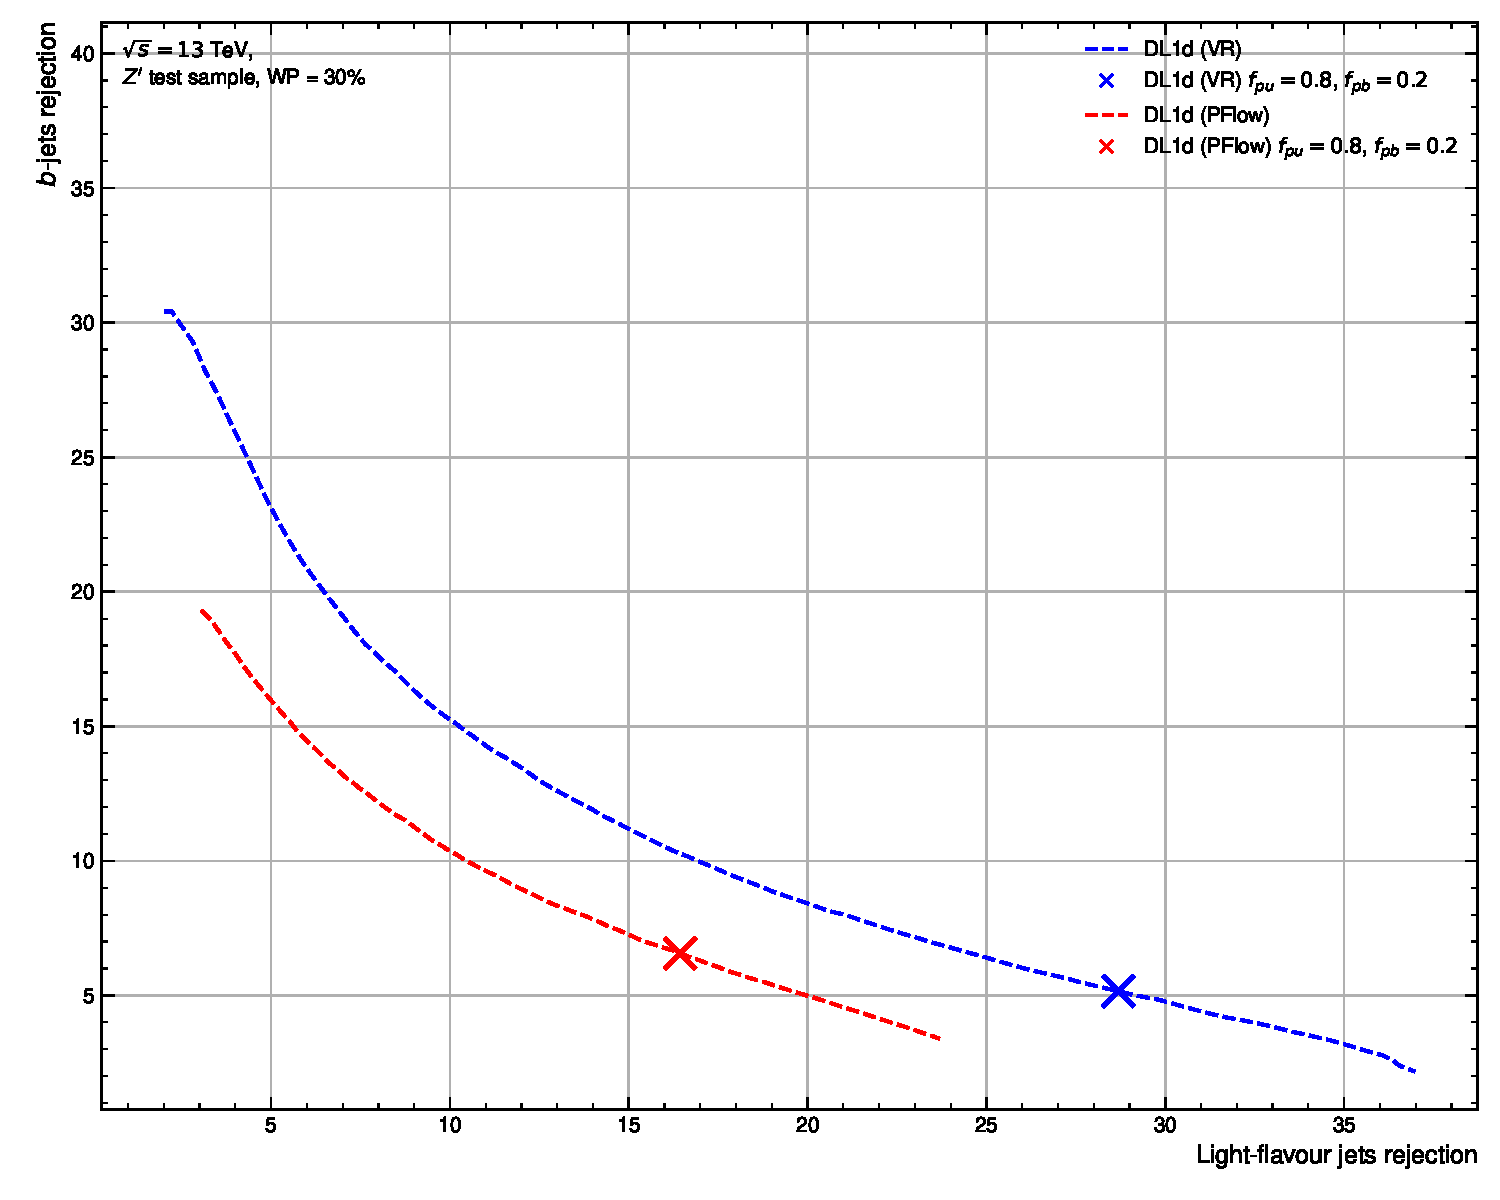
\includegraphics[width=0.32\textwidth]{Images/FTAG/VRDL1d/scansfraction/thesis_plot_frac_c/contour_fraction_zpext_2000.pdf}
    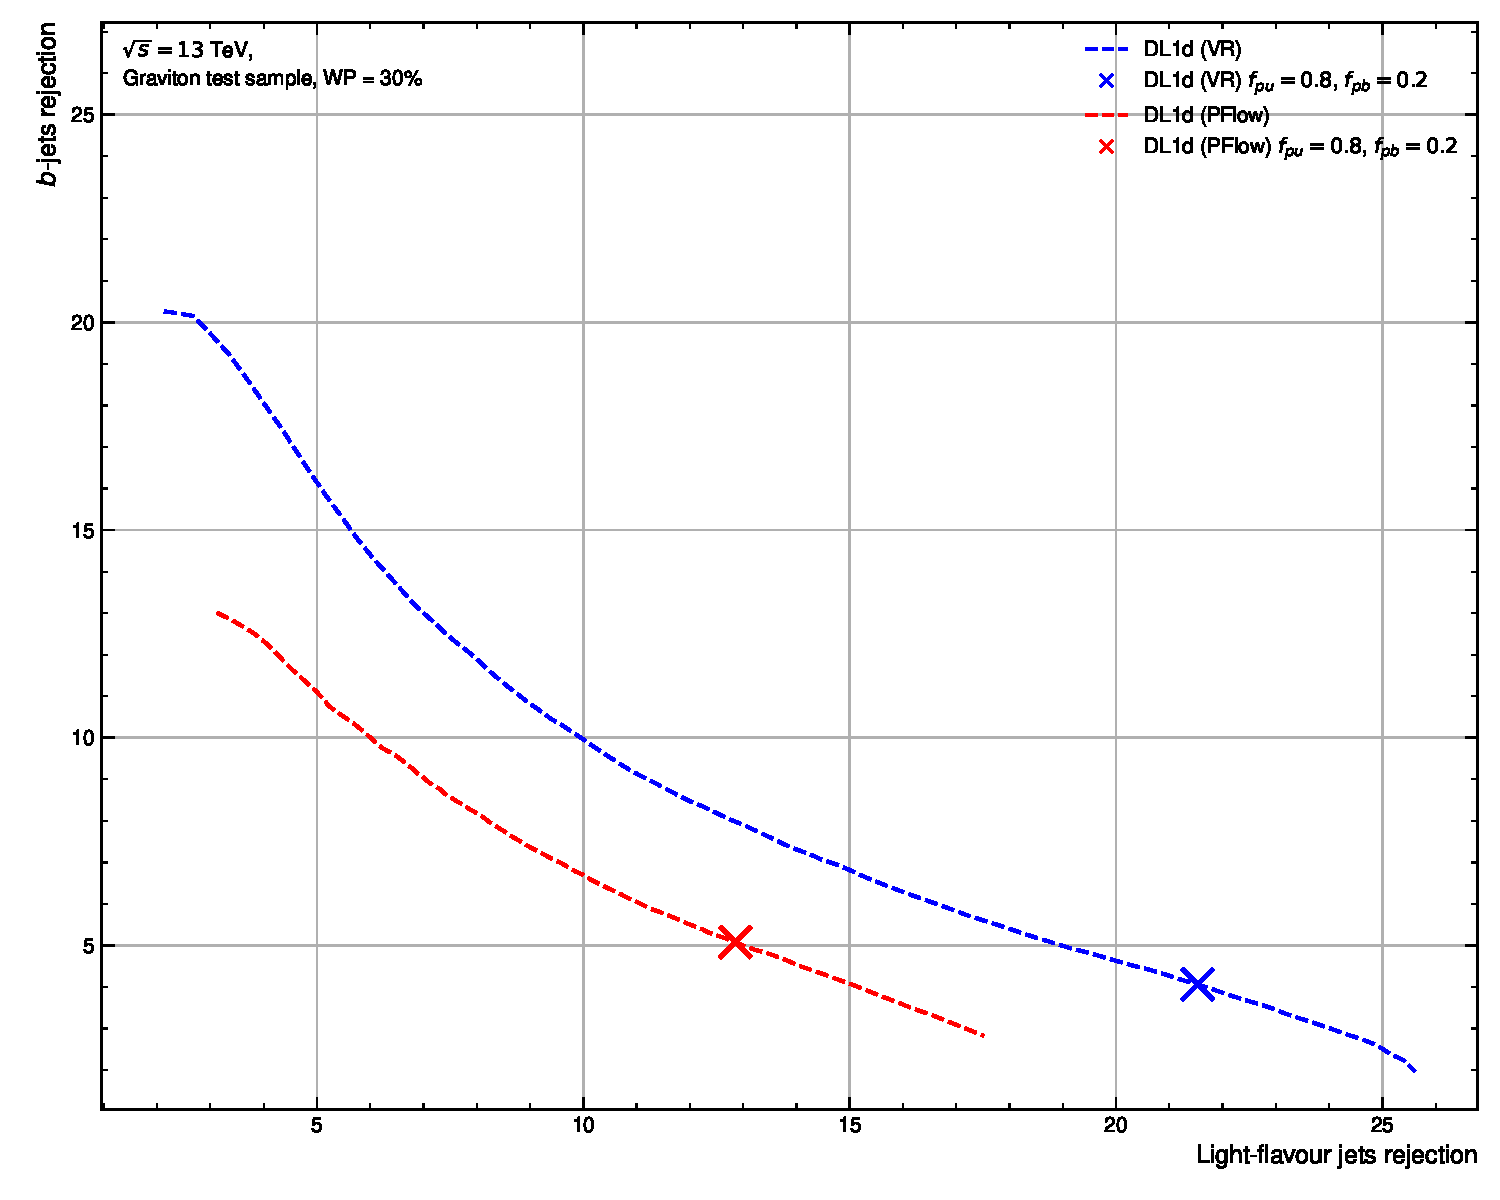
\includegraphics[width=0.32\textwidth]{Images/FTAG/VRDL1d/scansfraction/thesis_plot_frac_c/contour_fraction_graviton_2000.pdf}
    \caption{Flavour fraction $f_b^c$ for $c$-tagging scans.} 
    \label{fig:DL1dVRscanfc}
\end{subfigure}
  \caption{The flavour fractions scans of the VR- and PFlow-trained DL1d model in blue and red respectively: left is $t\bar{t}$, centre $Z'$, and right the graviton test samples. The chosen values are marked on the curves, displaying on the $y$-axis the $c$-rejection ($b$-rejection) for $b$-tagging ($c$-tagging) vs the light-rejection on the $x$ axis at a fixed working point of 77\% (33\%). Increasing $f_c$ or $f_b$ shifts the marker upwards along the curves. }
  \label{apfig:DL1dVRscanf}
\end{figure} 

\section{GN2 public plots}
A comparison of the global performance of this \gls{gn2} model to the \gls{dl1d} and \gls{gn1} models is displayed in the $b$- and $c$-tagging \gls{roc} curves of Figures \ref{fig:GN2rocb} and \ref{fig:GN2rocc}. These results are taken from Ref \cite{ATL-PLOT-FTAG-2023-01}, for which the \gls{dl1d} model was retrained on the same dataset as \gls{gn2}, and the \gls{dl1r} and \gls{gn1} models are taken from Chapter \ref{chap-GN1}. \gls{gn2} delivers yet another significant boost to performance, drasticaly surpassing the \gls{gn1} rejections at all efficiencies considered. The largest improvement is again obtained at lower $b$-jet efficiencies. Compared to \gls{gn1}, \gls{gn2} delivers $\times 1.5$ ($\times 1.7$) the $c$-rejection (light-rejection) on $t\bar{t}$ at the 70\% $b$-tagging \gls{wp} and $\times 1.75$ ($\times 1.2$) on $Z'$ at 30\% \gls{wp}. With respect to \gls{dl1d}, the gains in $c$-rejection (light-rejection) are respectively close to $\times 3$ ($\times 2$) for $t\bar{t}$ and $\times 3.4$ ($\times 4$) on $Z'$. 

\begin{center}
    \vspace{-1.cm}
    \begin{figure}[h!]
    \centerline{
    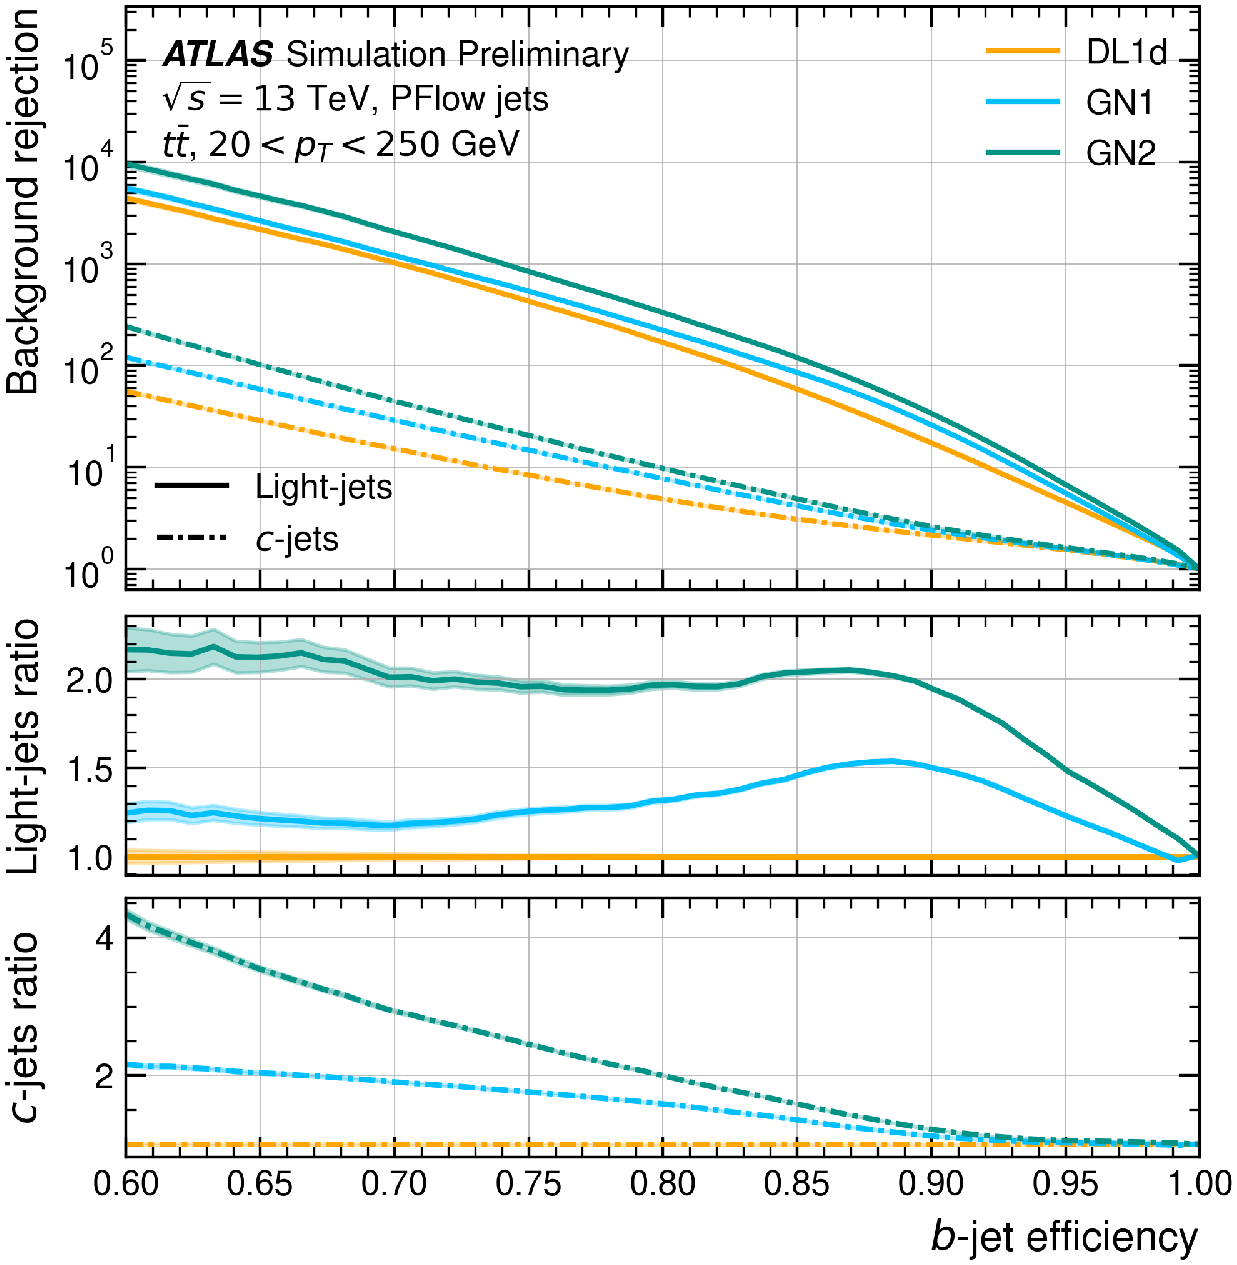
\includegraphics[width=0.48\textwidth]{Images/FTAG/GN/GN2/ROCpublic/ttb.png}
    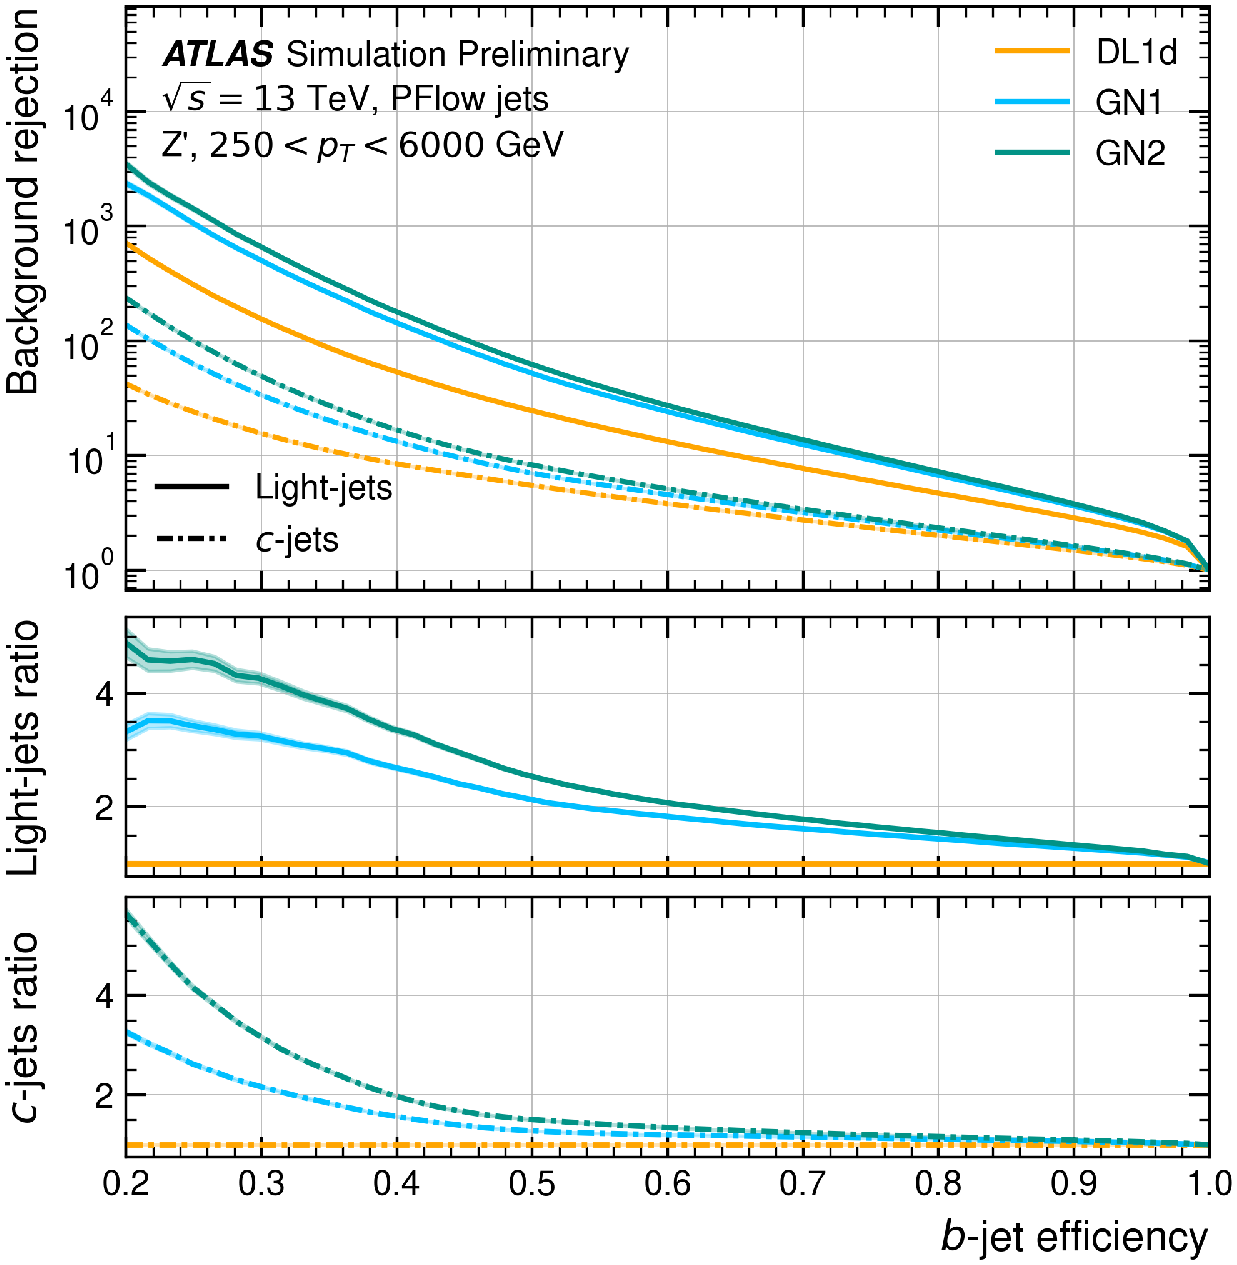
\includegraphics[width=0.48\textwidth]{Images/FTAG/GN/GN2/ROCpublic/zpb.png}
    }
    \caption{The $c$- and light-rejections as a function of the $b$-jet tagging efficiency in the $t\bar{t}$ with $20 < p_T < 250$ GeV (left) and $Z'$ with $250 < p_T < 6000$ GeV (right) test samples, from \cite{ATL-PLOT-FTAG-2023-01}. Models compared are DL1d in orange, GN1 in turquoise, and GN2 in blue. The bottom plots show the ratio with respect to the DL1d performance. Flavour fractions are set at $f^b_c = 0.018$ for DL1d, 0.05 for GN1, and 0.1 for GN2. Shaded regions represent the binominal error band.}
    \label{apfig:GN2rocb}
    \bigskip
    \centerline{
    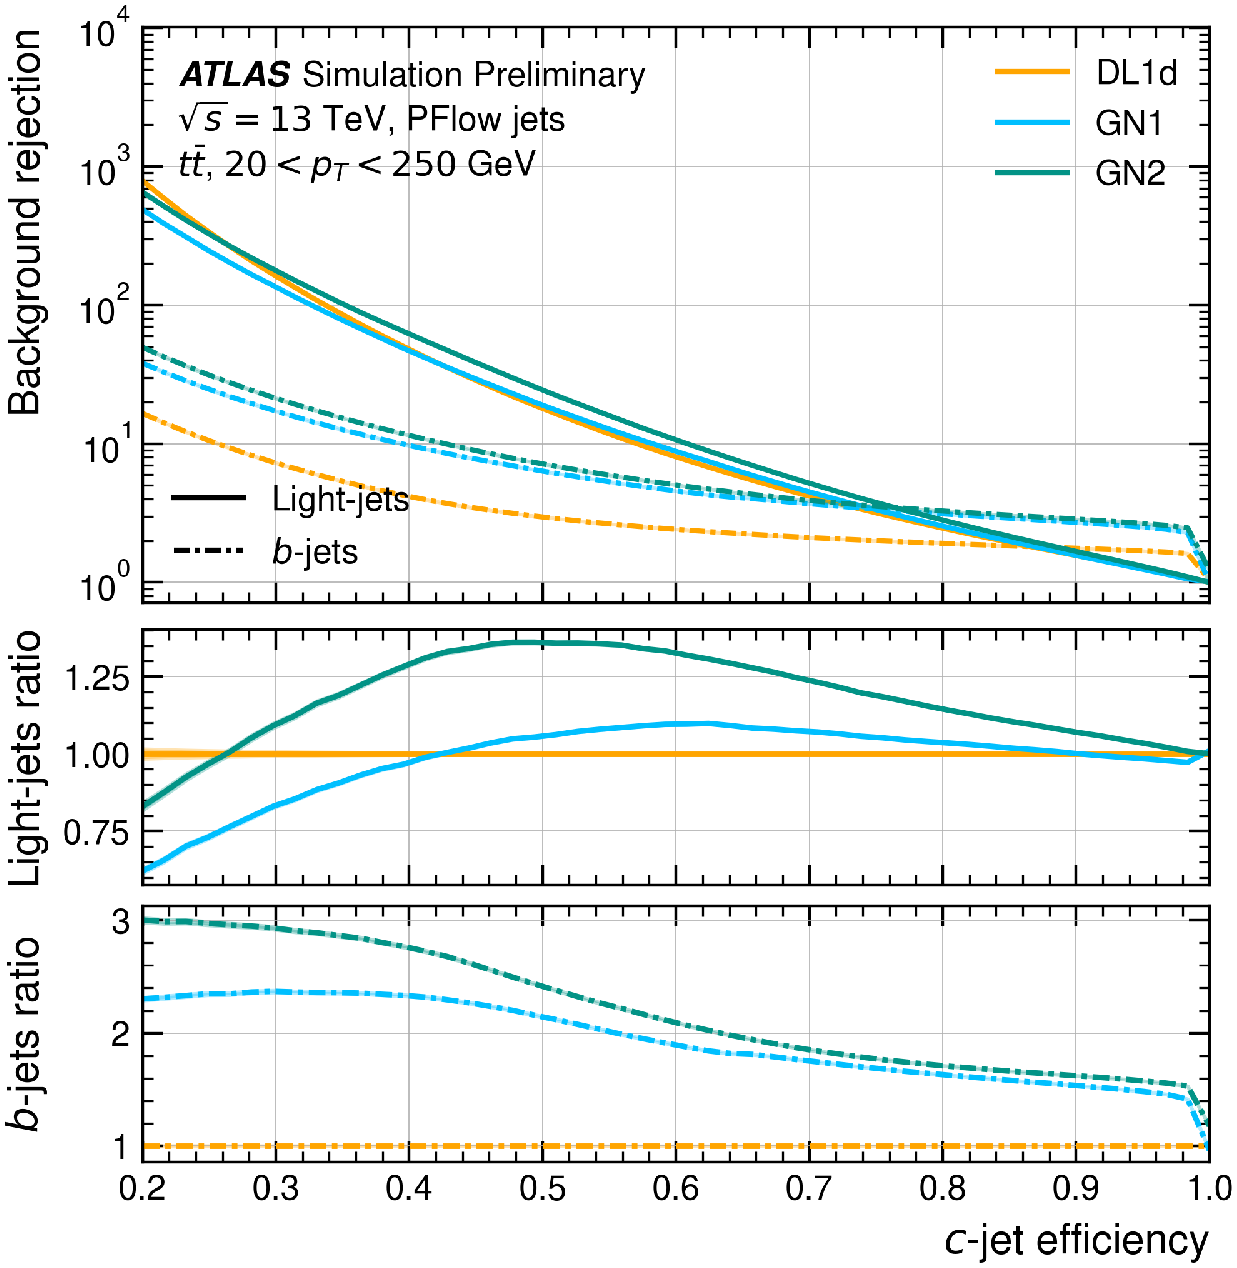
\includegraphics[width=0.48\textwidth]{Images/FTAG/GN/GN2/ROCpublic/ttc.png}
    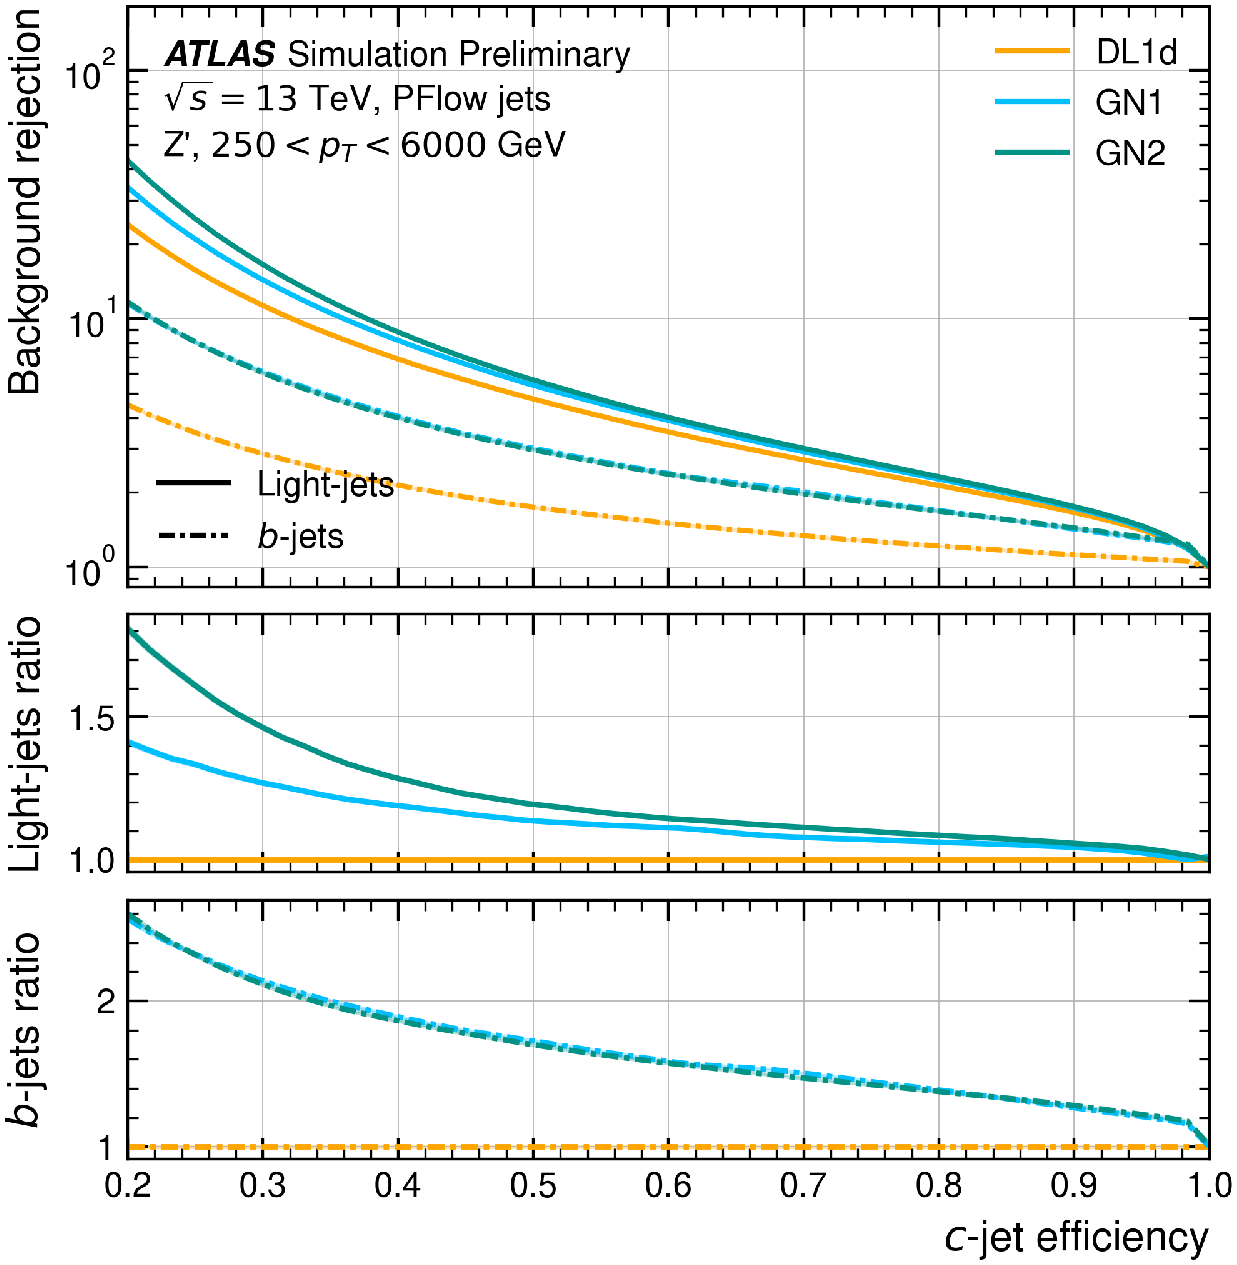
\includegraphics[width=0.48\textwidth]{Images/FTAG/GN/GN2/ROCpublic/zpc.png}
    }
    \caption{The $b$- and light-rejections as a function of the $c$-jet tagging efficiency in the $t\bar{t}$ with $20 < p_T < 250$ GeV (left) and $Z'$ with $250 < p_T < 6000$ GeV (right) test samples, from \cite{ATL-PLOT-FTAG-2023-01}. Models compared are DL1d in orange, GN1 in turquoise, and GN2 in blue. The bottom plots show the ratio with respect to the DL1d performance. Flavour fractions are set at $f^c_b = 0.2$ for all taggers. Shaded regions represent the binominal error band.}
    \label{apfig:GN2rocc}
    \end{figure}
\end{center}

Turning to $c$-tagging, a similar large performance gained is obtained by the new \gls{gnn} family over \gls{dl1d}, although the change on the $t\bar{t}$ is more impressive for the $b$-jet ratio than for light-jet. This indicates a non-optimal choice for the flavour fraction $f^c_b$, which was set at 0.2 for all models.

\section{GN2 supporting plots}\label{app-GN2sup}
This section presents more plots in support of Chapter \ref{chap-GN2}. Figure \ref{apfig:GNxptc_eff} presents the $c$-tagging efficiency per bin for an overall $c$-tagging working point of 30\% per region displayed. 

\begin{figure}[h!]
    \centering
    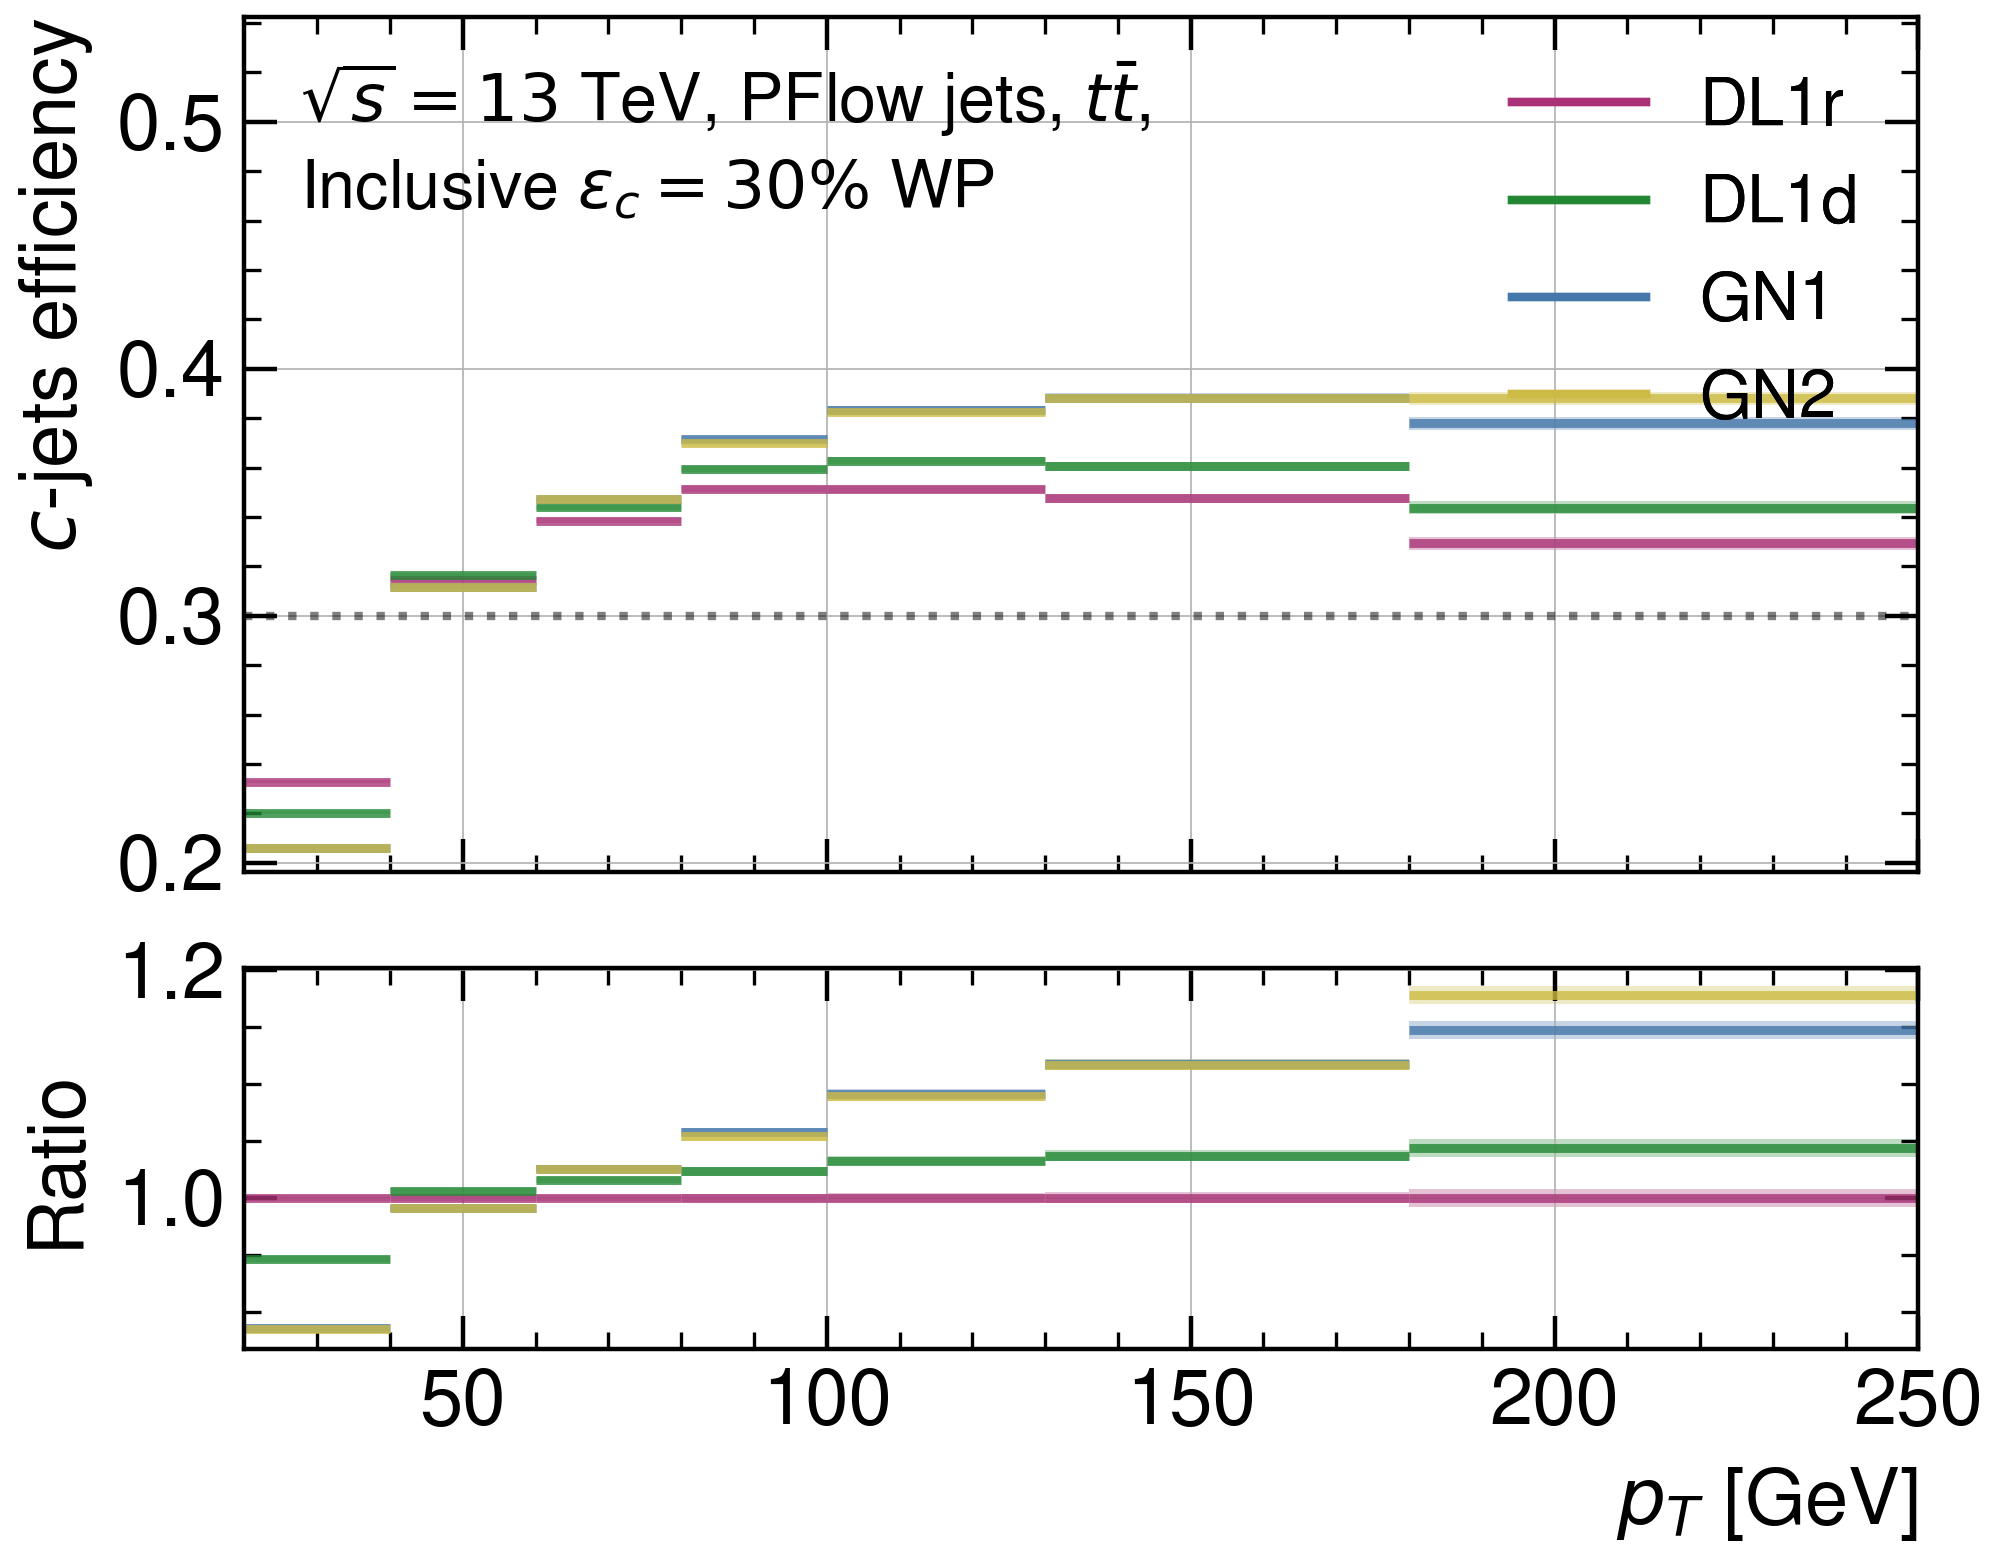
\includegraphics[width=0.48\textwidth]{Images/FTAG/GN/GN2/pt_plots/pt_ttbar_c_eff.png}
    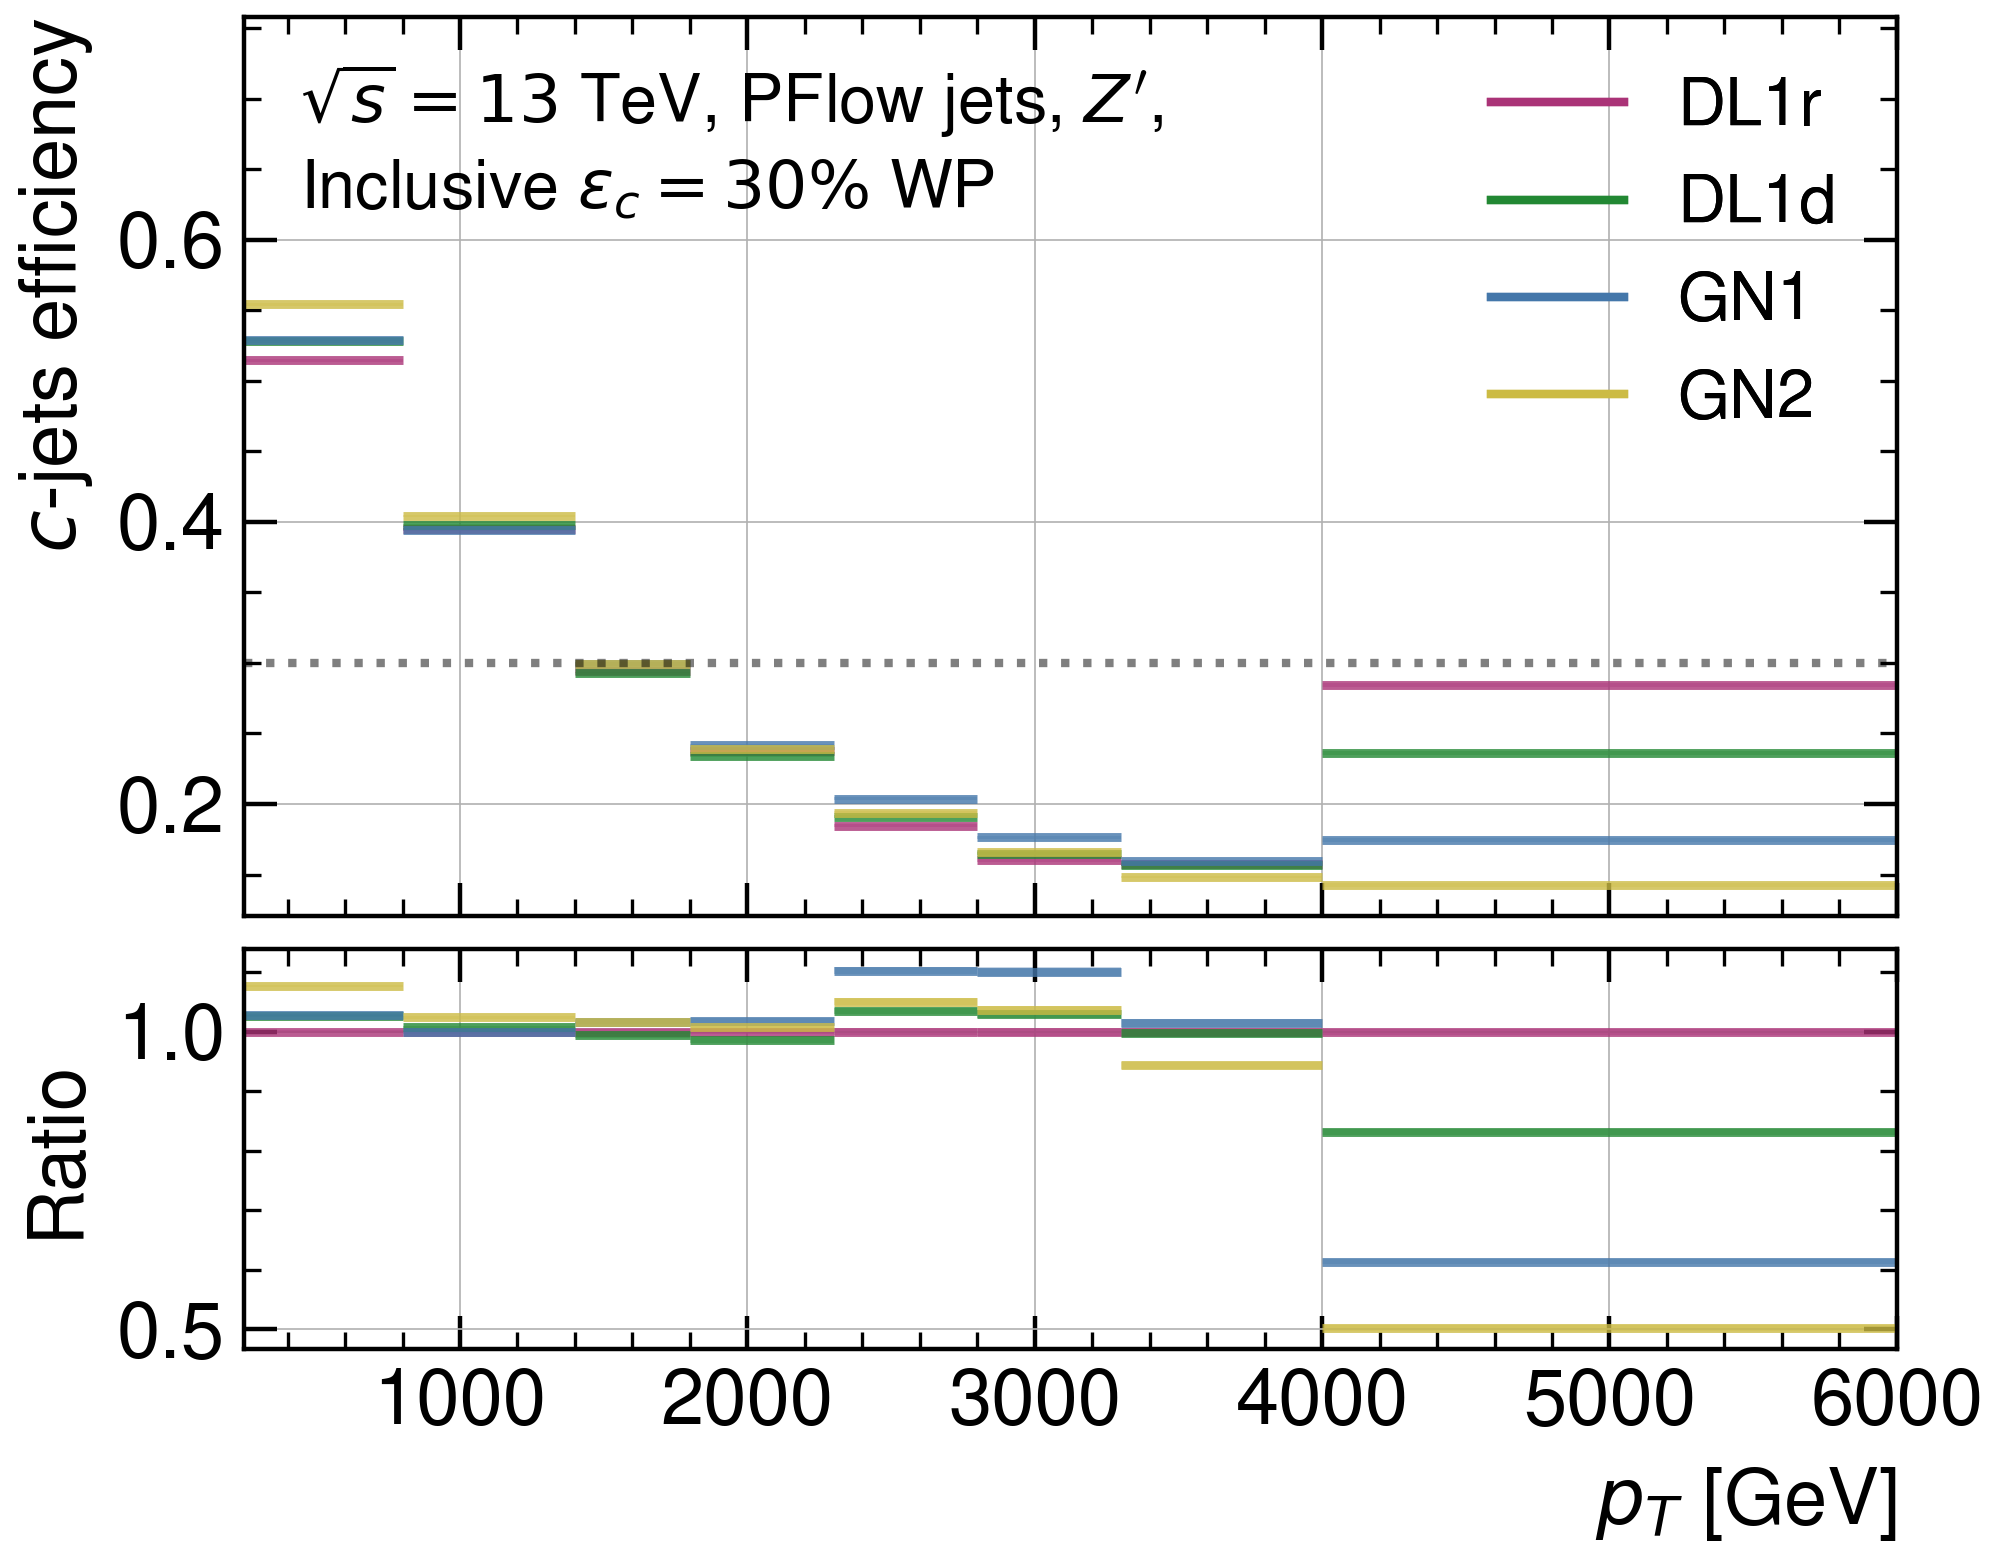
\includegraphics[width=0.48\textwidth]{Images/FTAG/GN/GN2/pt_plots/pt_zp_c_eff.png}
    \caption{Comparing the different models $c$-tagging efficiency as a function of jet $p_T$ for the inclusive $c$-tagging 30\% working point on the $t\bar{t}$ (left) and $Z'$ (right). The flavour fraction is set at $f^c_b = 0.2$ for all taggers.}
    \label{apfig:GNxptc_eff}
\end{figure} 

Figure \ref{apfig:GNxptc_efffixedl} presents the $c$-tagging efficiency per bin for a per bin light-rejection of 50 for $t\bar{t}$ and 10 for $Z'$. The \gls{gn2} performance dominates across the board, except for the highest energy bin of the $Z'$. 

\begin{figure}[h!]
    \centering
    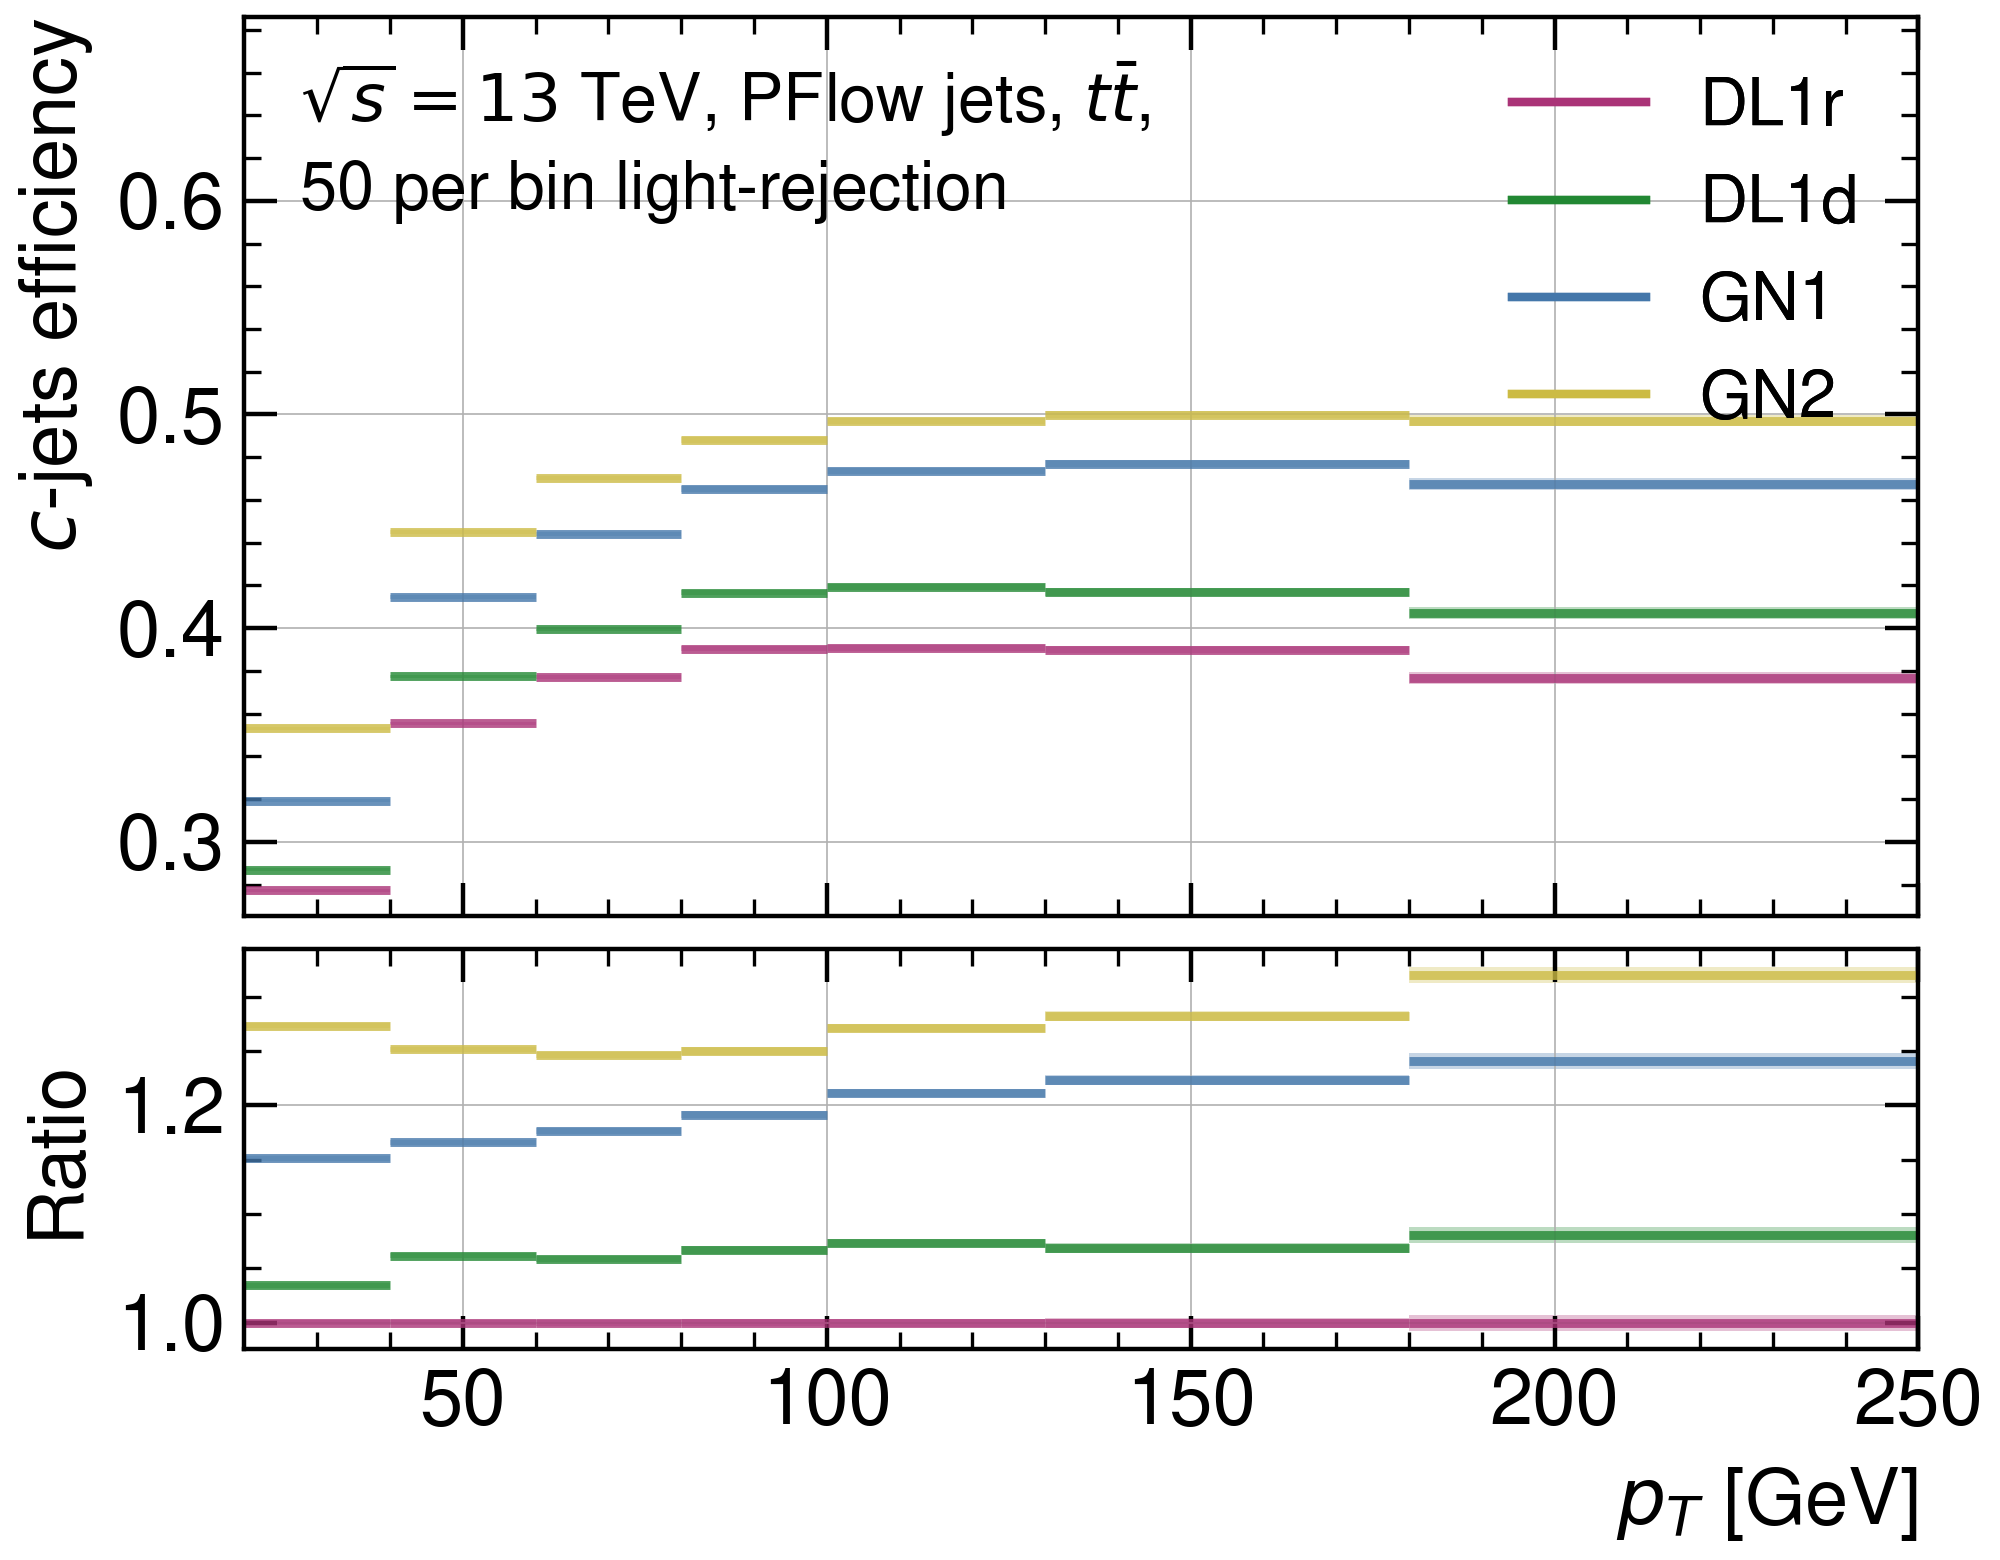
\includegraphics[width=0.48\textwidth]{Images/FTAG/GN/GN2/pt_plots/pt_ttbar_c_eff_fixedlight.png}
    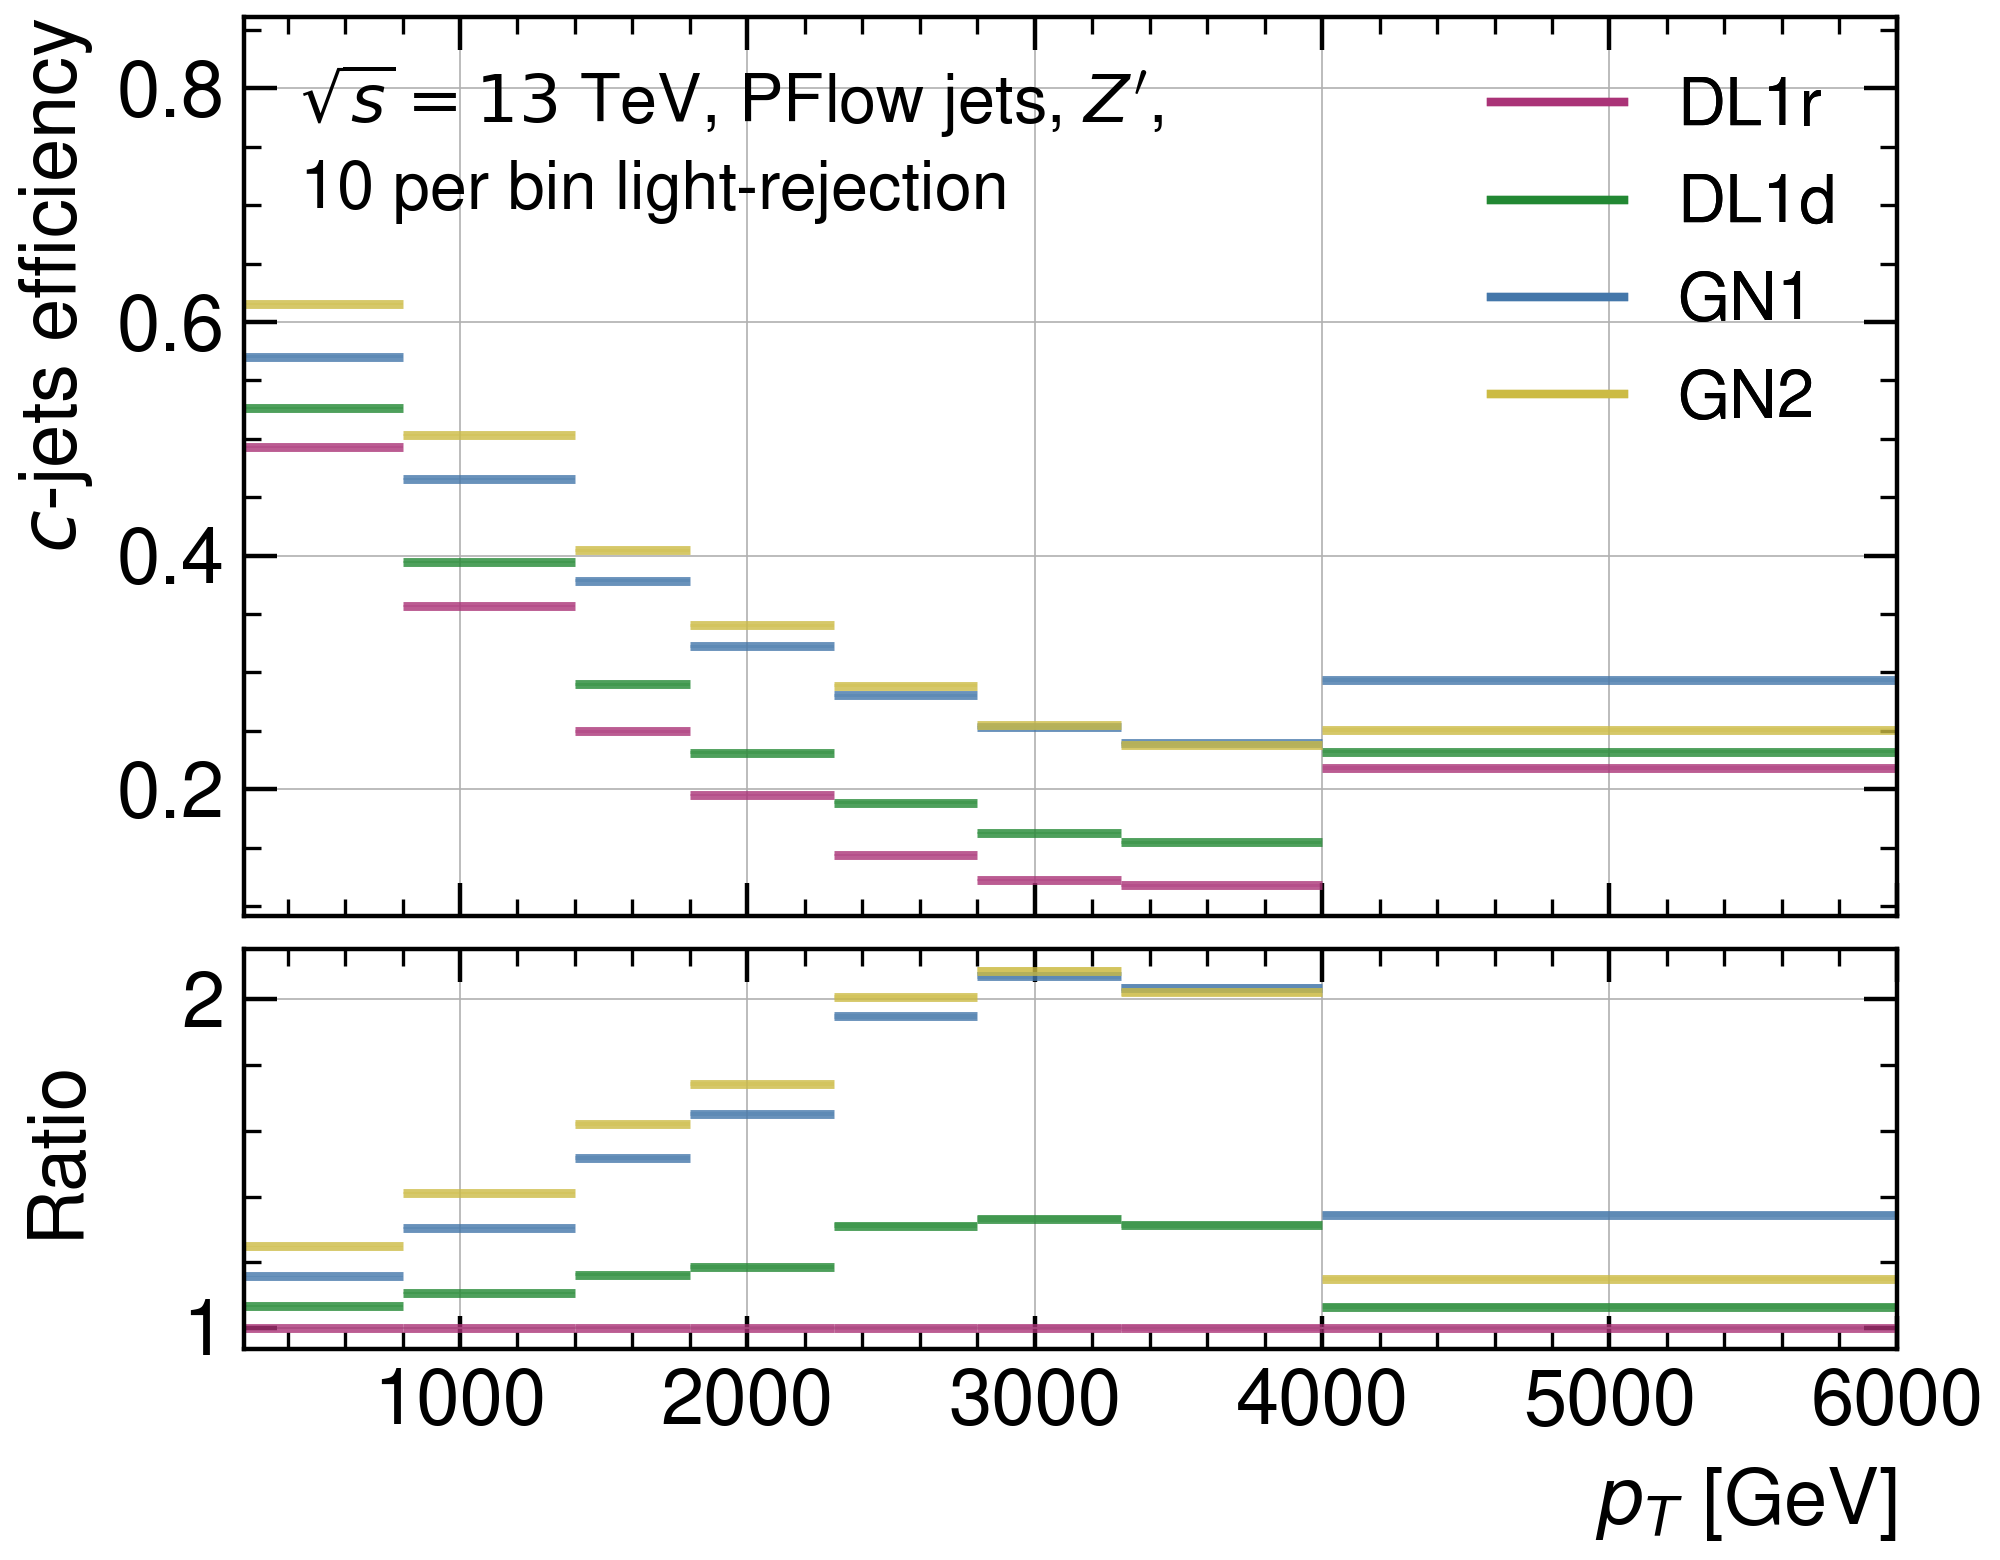
\includegraphics[width=0.48\textwidth]{Images/FTAG/GN/GN2/pt_plots/pt_zp_c_eff_fixedlight.png}
    \caption{Comparing the different models $c$-tagging efficiency as a function of jet $p_T$ at a fixed light-jet rejection per bin of 50 for the $t\bar{t}$ (left) and 10 for the $Z'$ (right) test samples. The flavour fraction is set at $f^c_b = 0.2$ for all taggers.}
    \label{apfig:GNxptc_efffixedl}
  \end{figure} 

Figures \ref{apfig:GNxptc_efffixedl} presents the $c$- and light-rejection at an inclusive 70\% $b$-tagging \gls{wp}. The equivalent information for $c$-tagging at a $c$-tagging \gls{wp} of 30\% is displayed in Figures \ref{apfig:GNxptc_brej} and \ref{apfig:GNxptc_urej} for $b$- and light-rejection. 
% Rej c - btagging
\begin{figure}[h!]
    \centering
    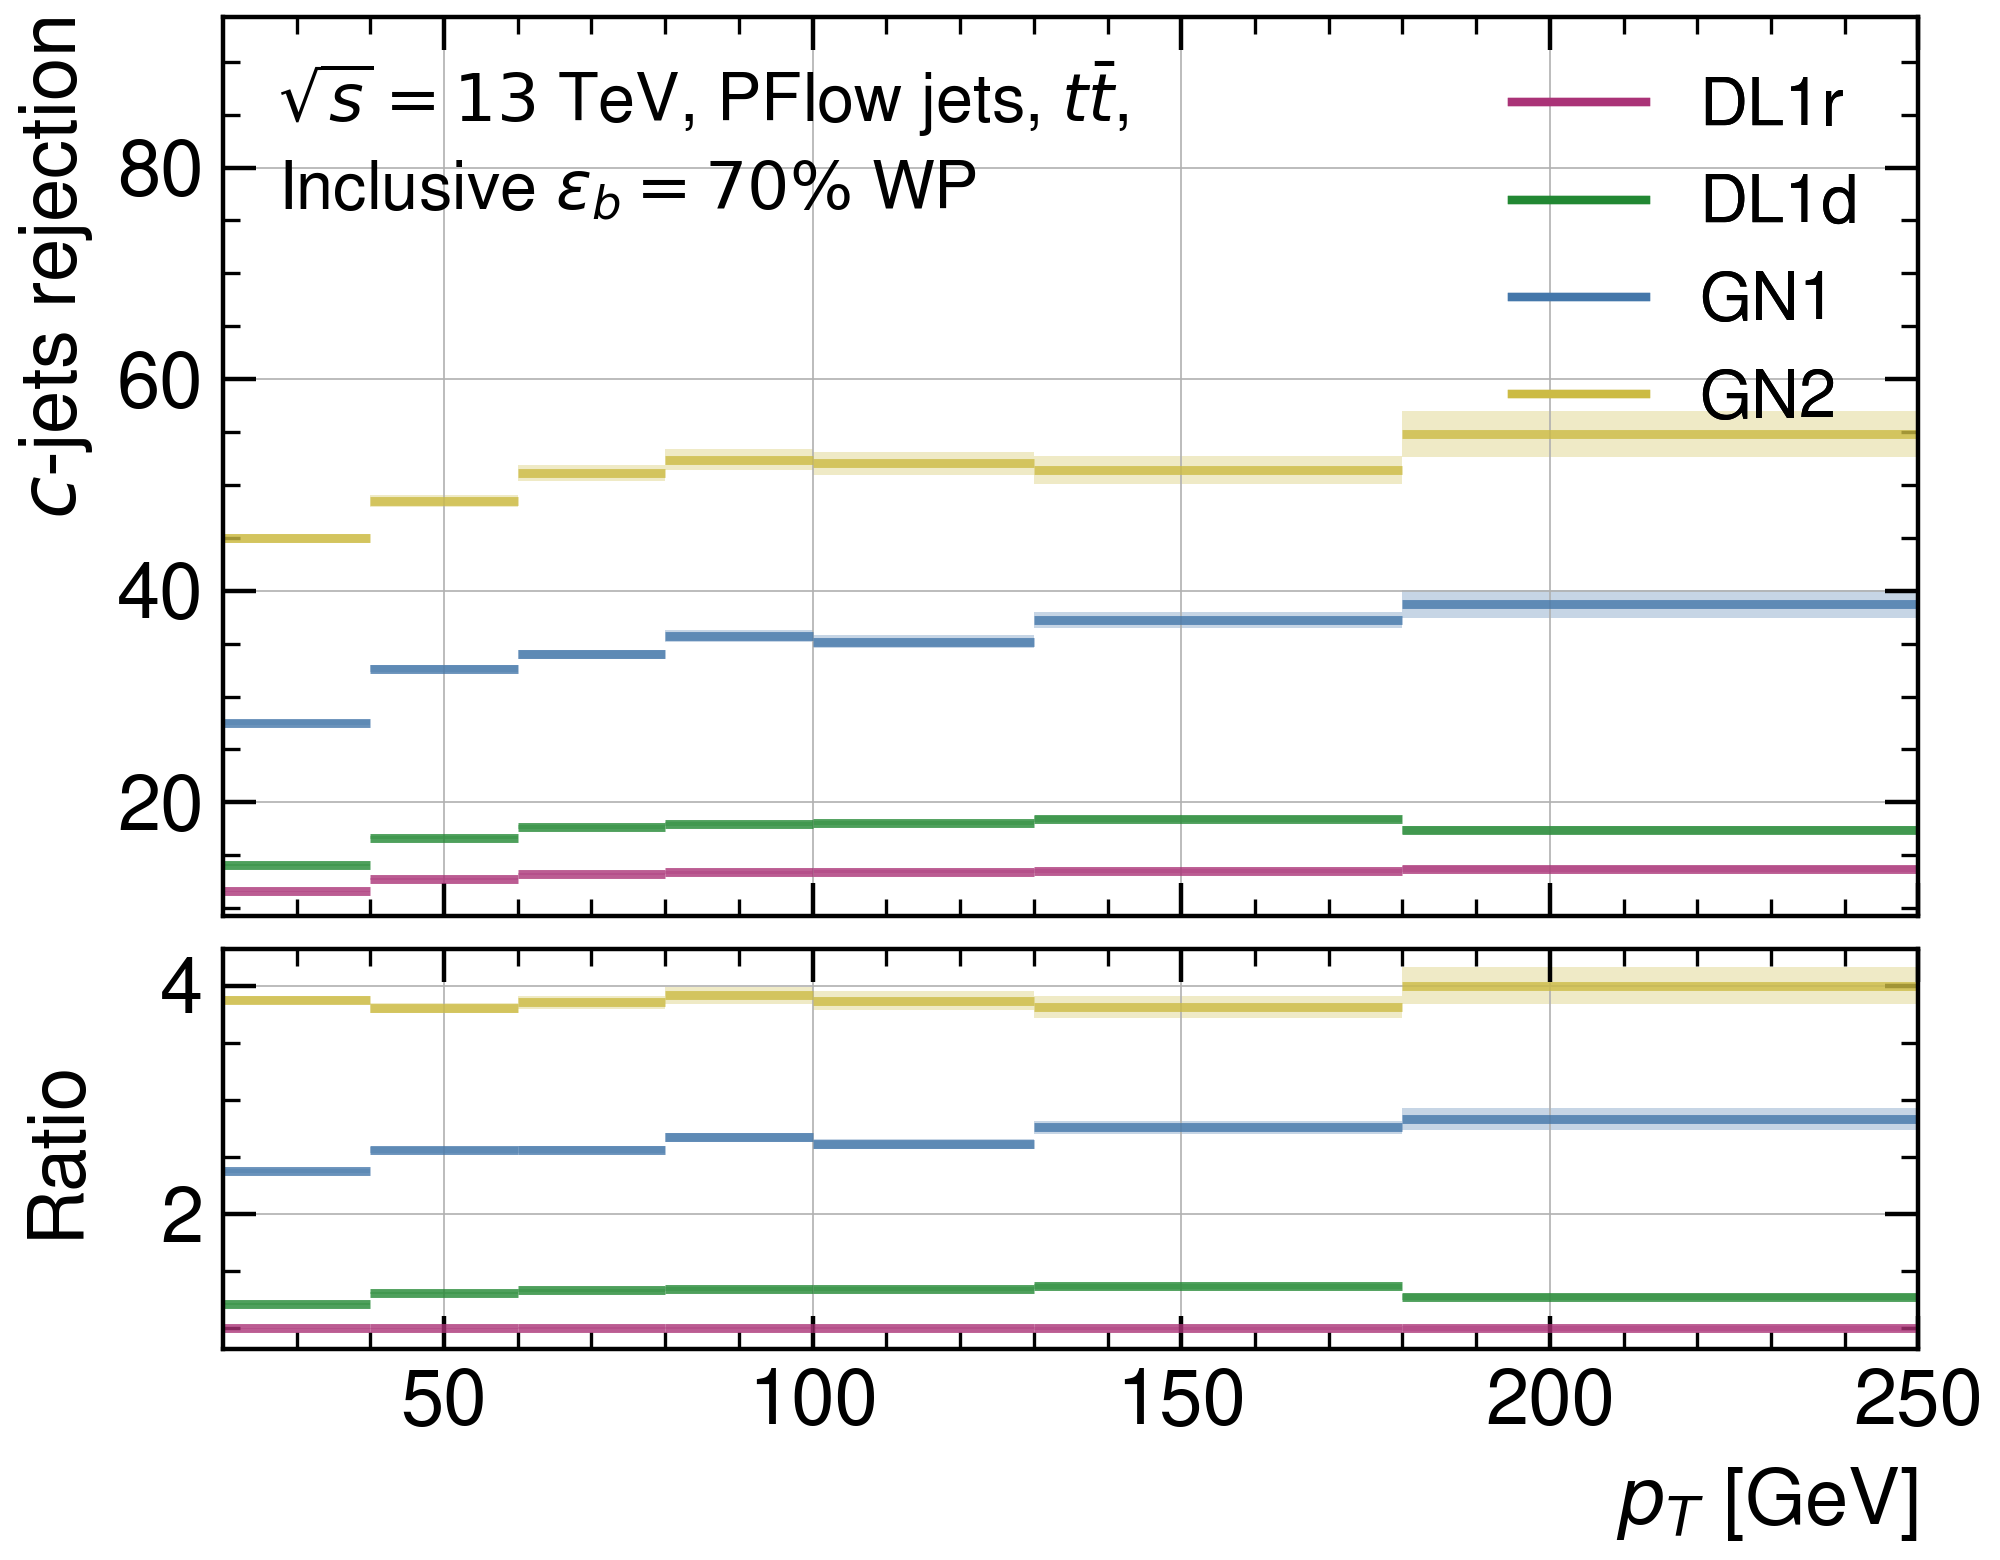
\includegraphics[width=0.48\textwidth]{Images/FTAG/GN/GN2/pt_plots/pt_ttbar_c_rej.png}
    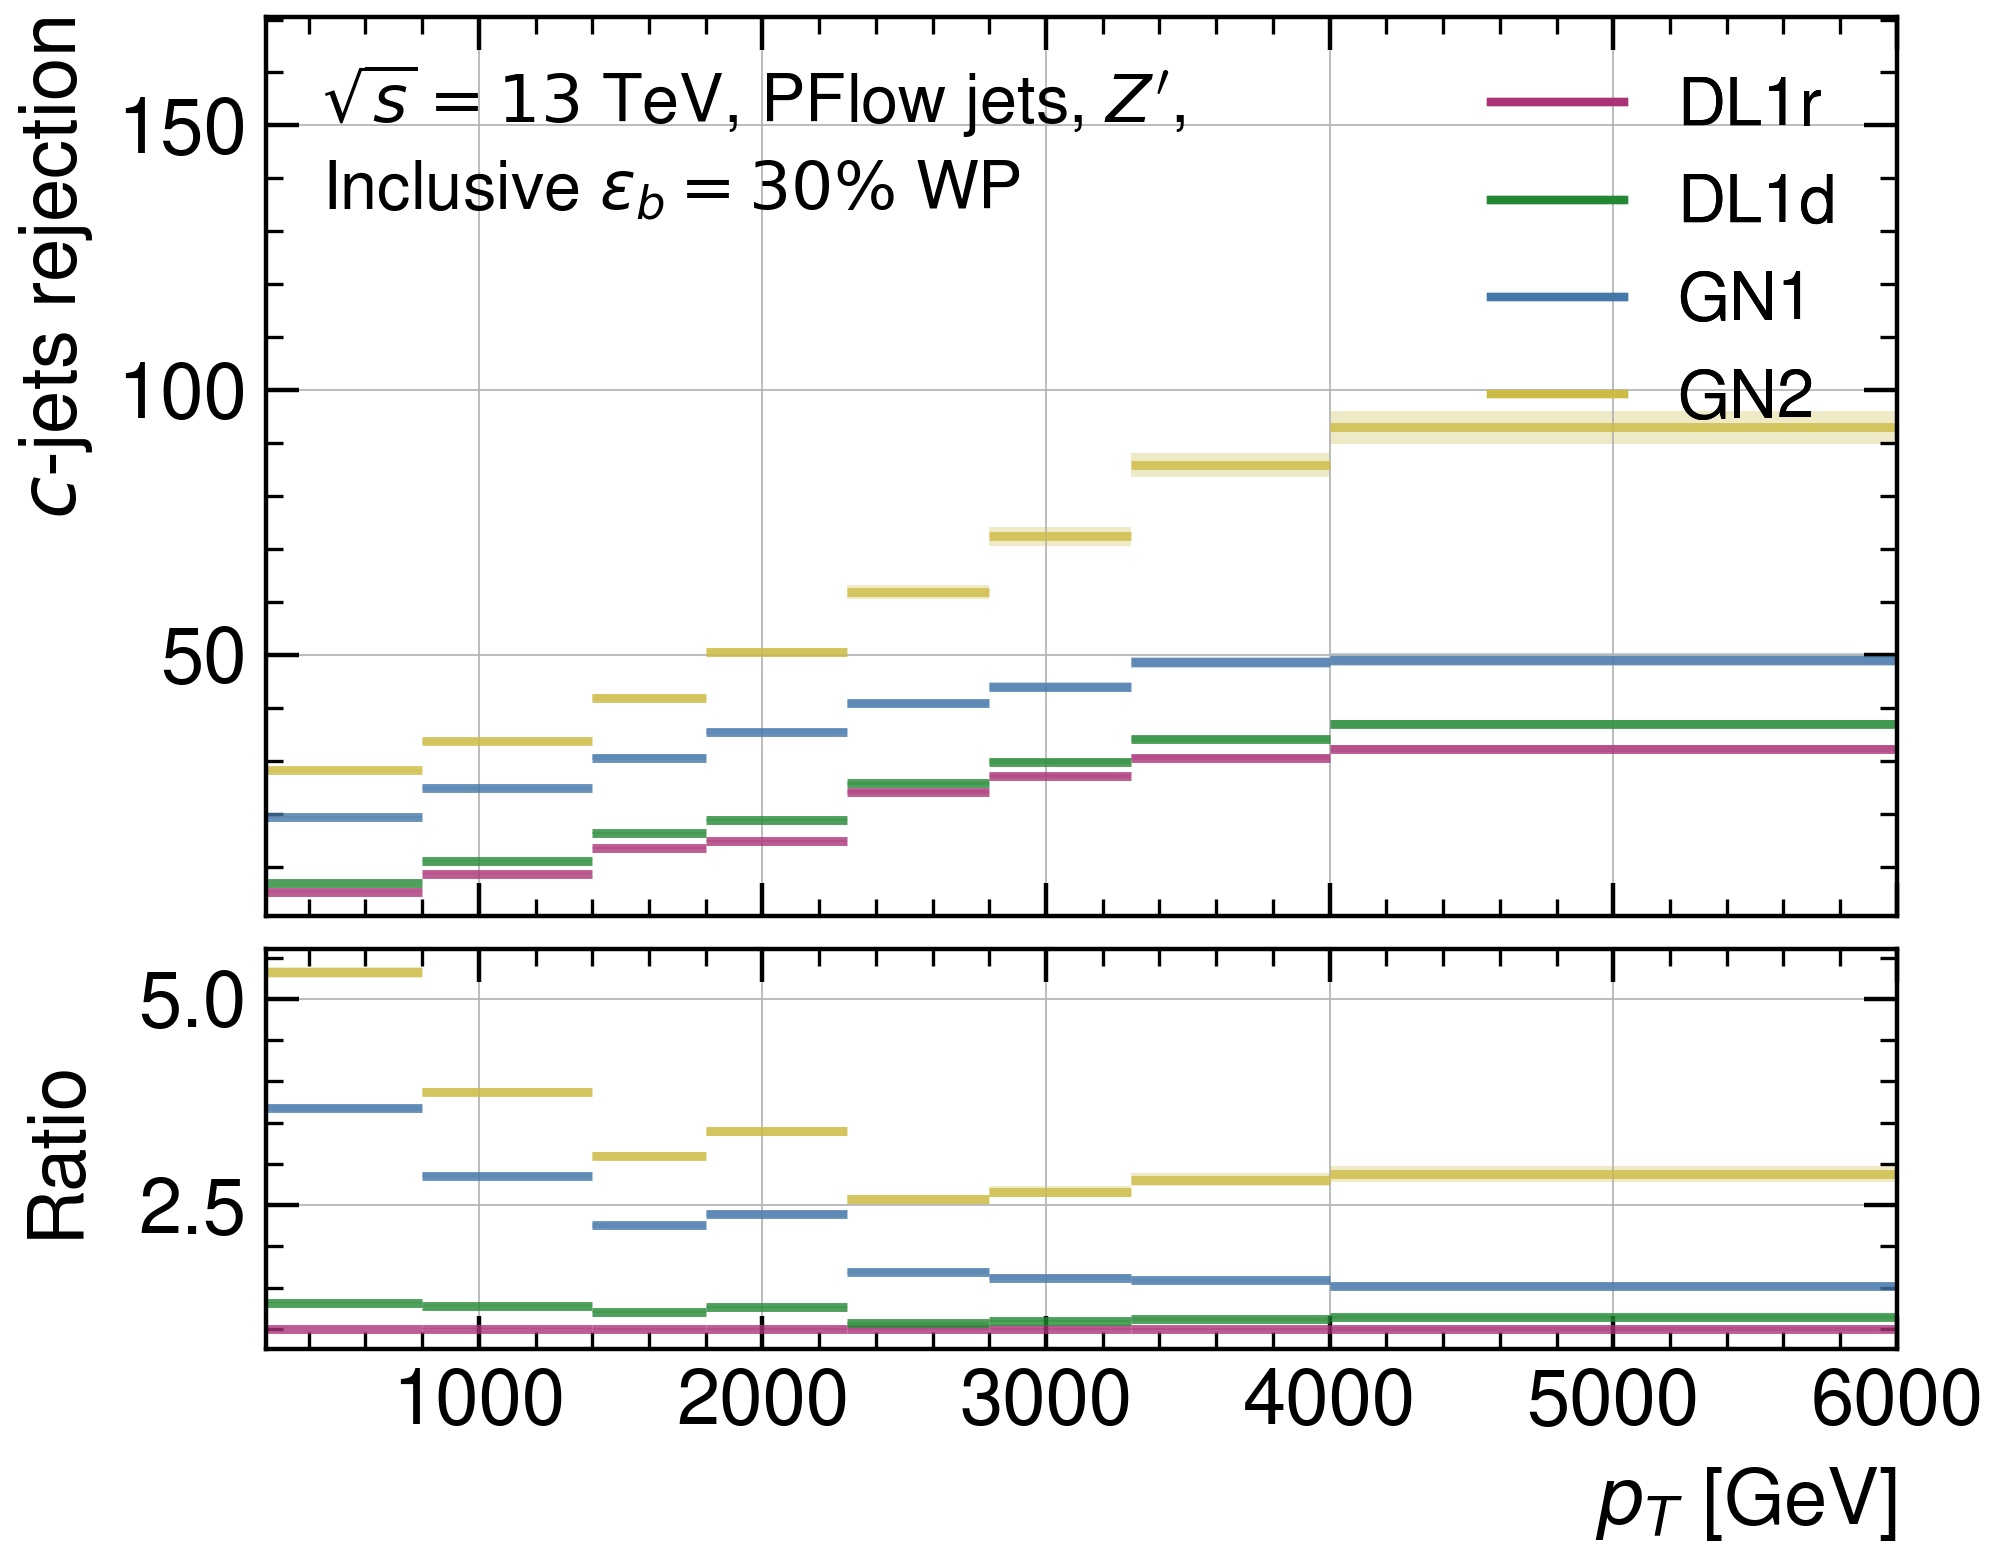
\includegraphics[width=0.48\textwidth]{Images/FTAG/GN/GN2/pt_plots/pt_zp_c_rej.png}
    \caption{Comparing the different models $c$-rejection as a function of jet $p_T$ for the $b$-tagging inclusive 70\% working point on the $t\bar{t}$ (left) and 30\% working point on $Z'$ (right). The flavour fraction is set at $f^b_c = 0.018$ for DL1r and DL1d, 0.05 for GN1, and 0.1 for GN2.}
    \label{apfig:GNxptb_crej}
  \end{figure} 
  
  % Rej light - btagging
  \begin{figure}[h!]
    \centering
    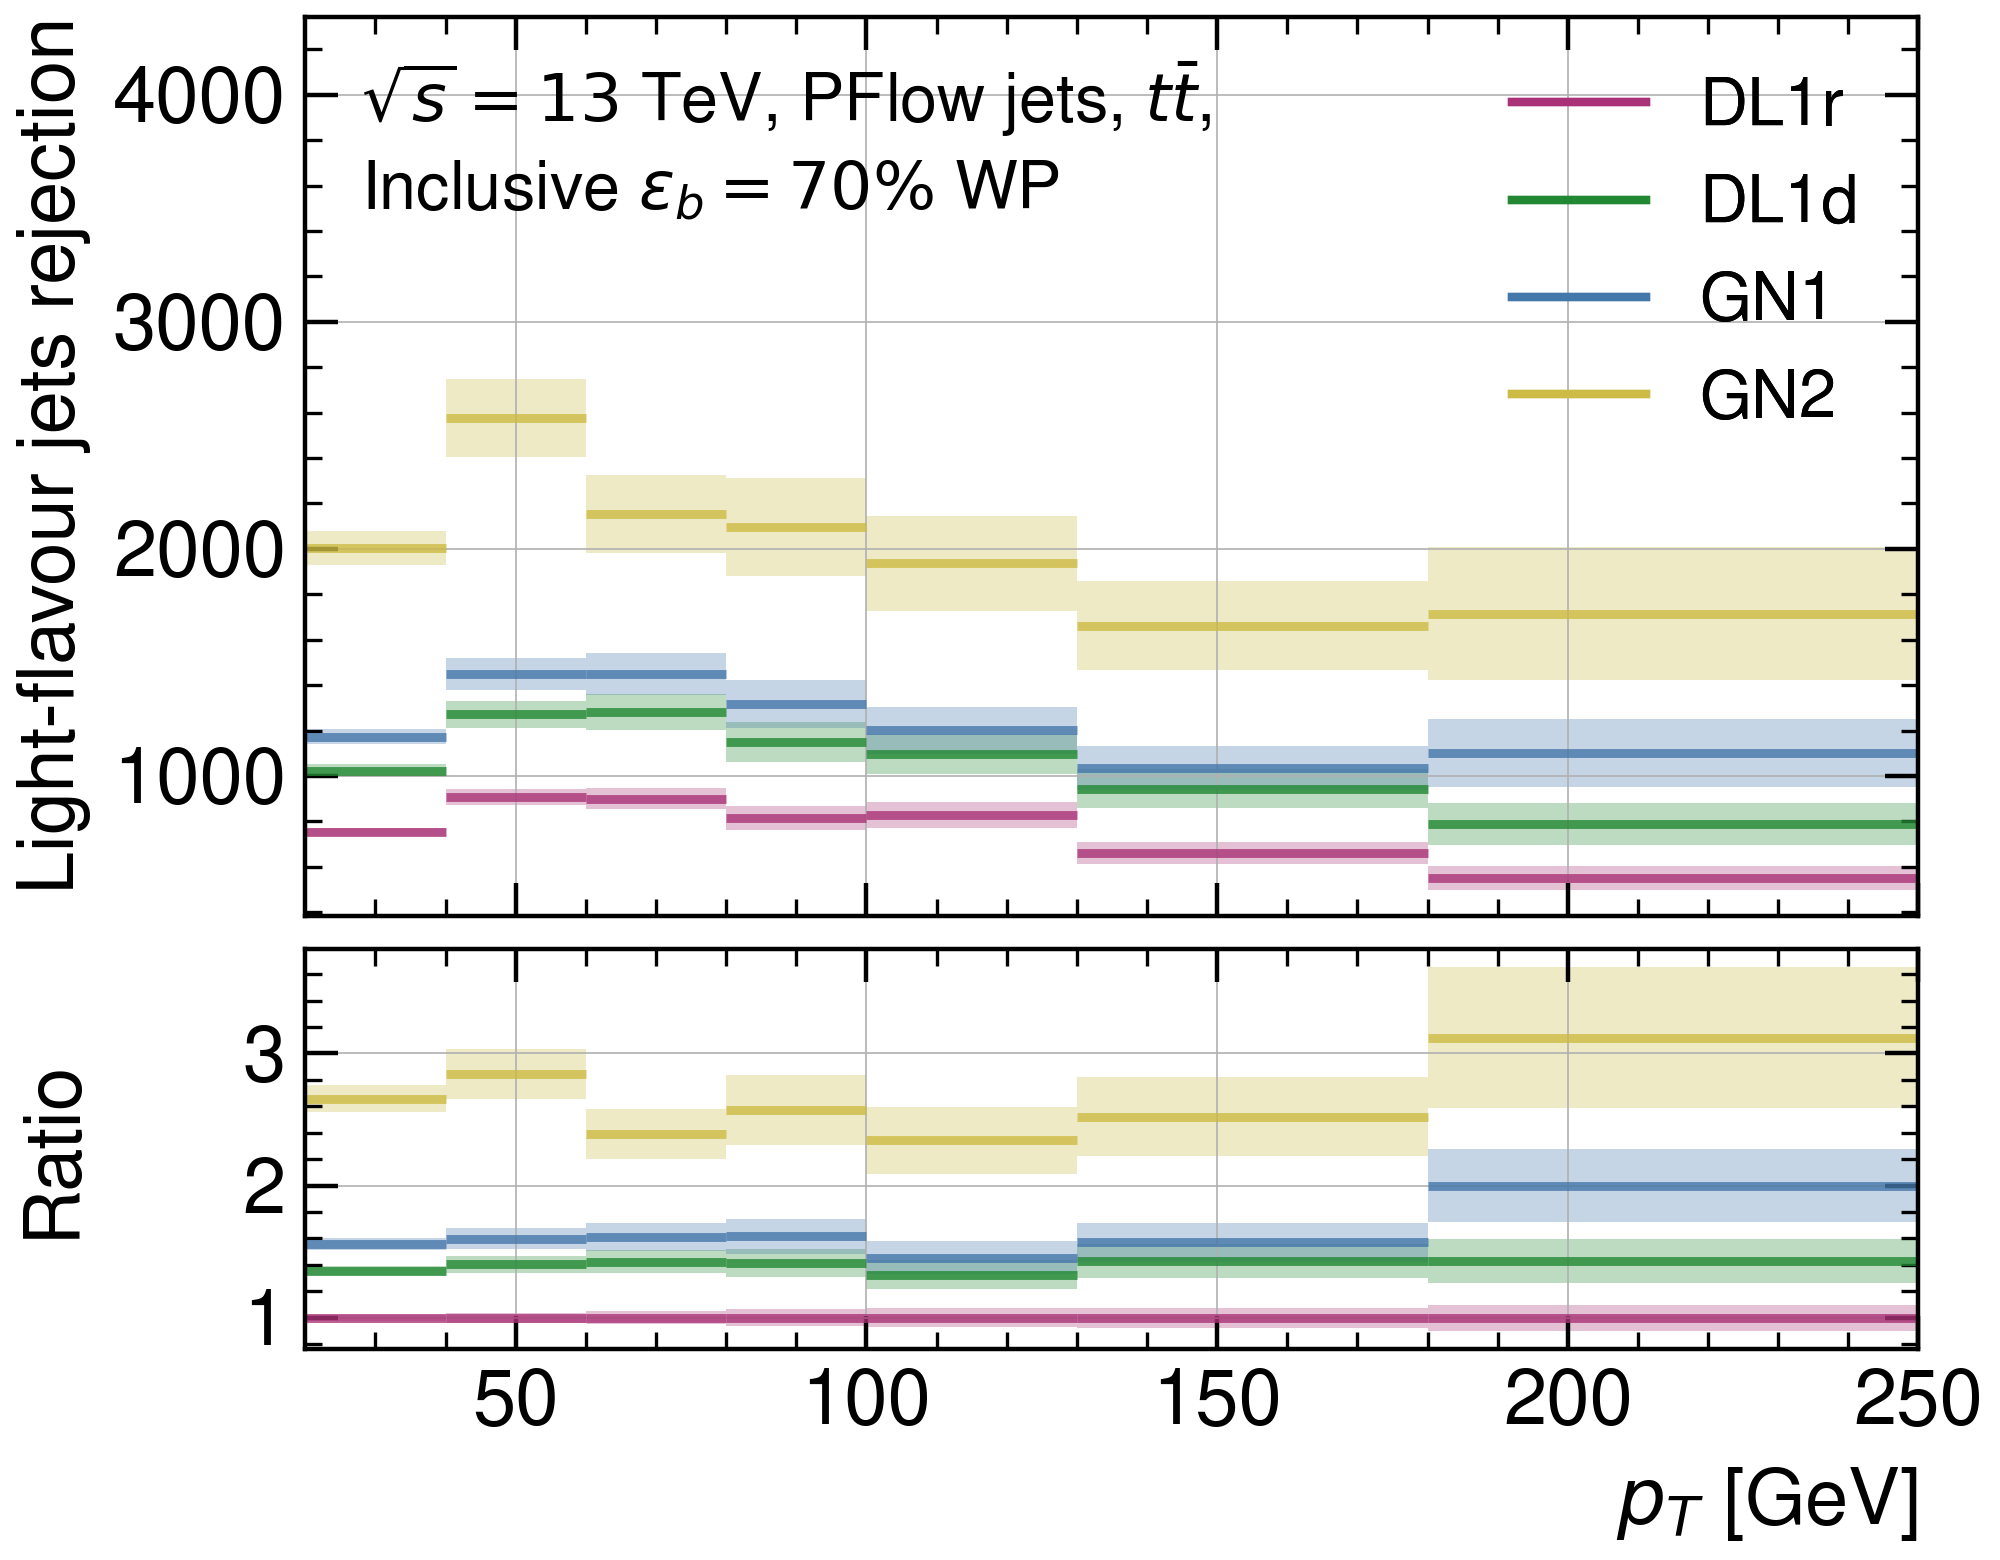
\includegraphics[width=0.48\textwidth]{Images/FTAG/GN/GN2/pt_plots/pt_ttbar_light_rej.png}
    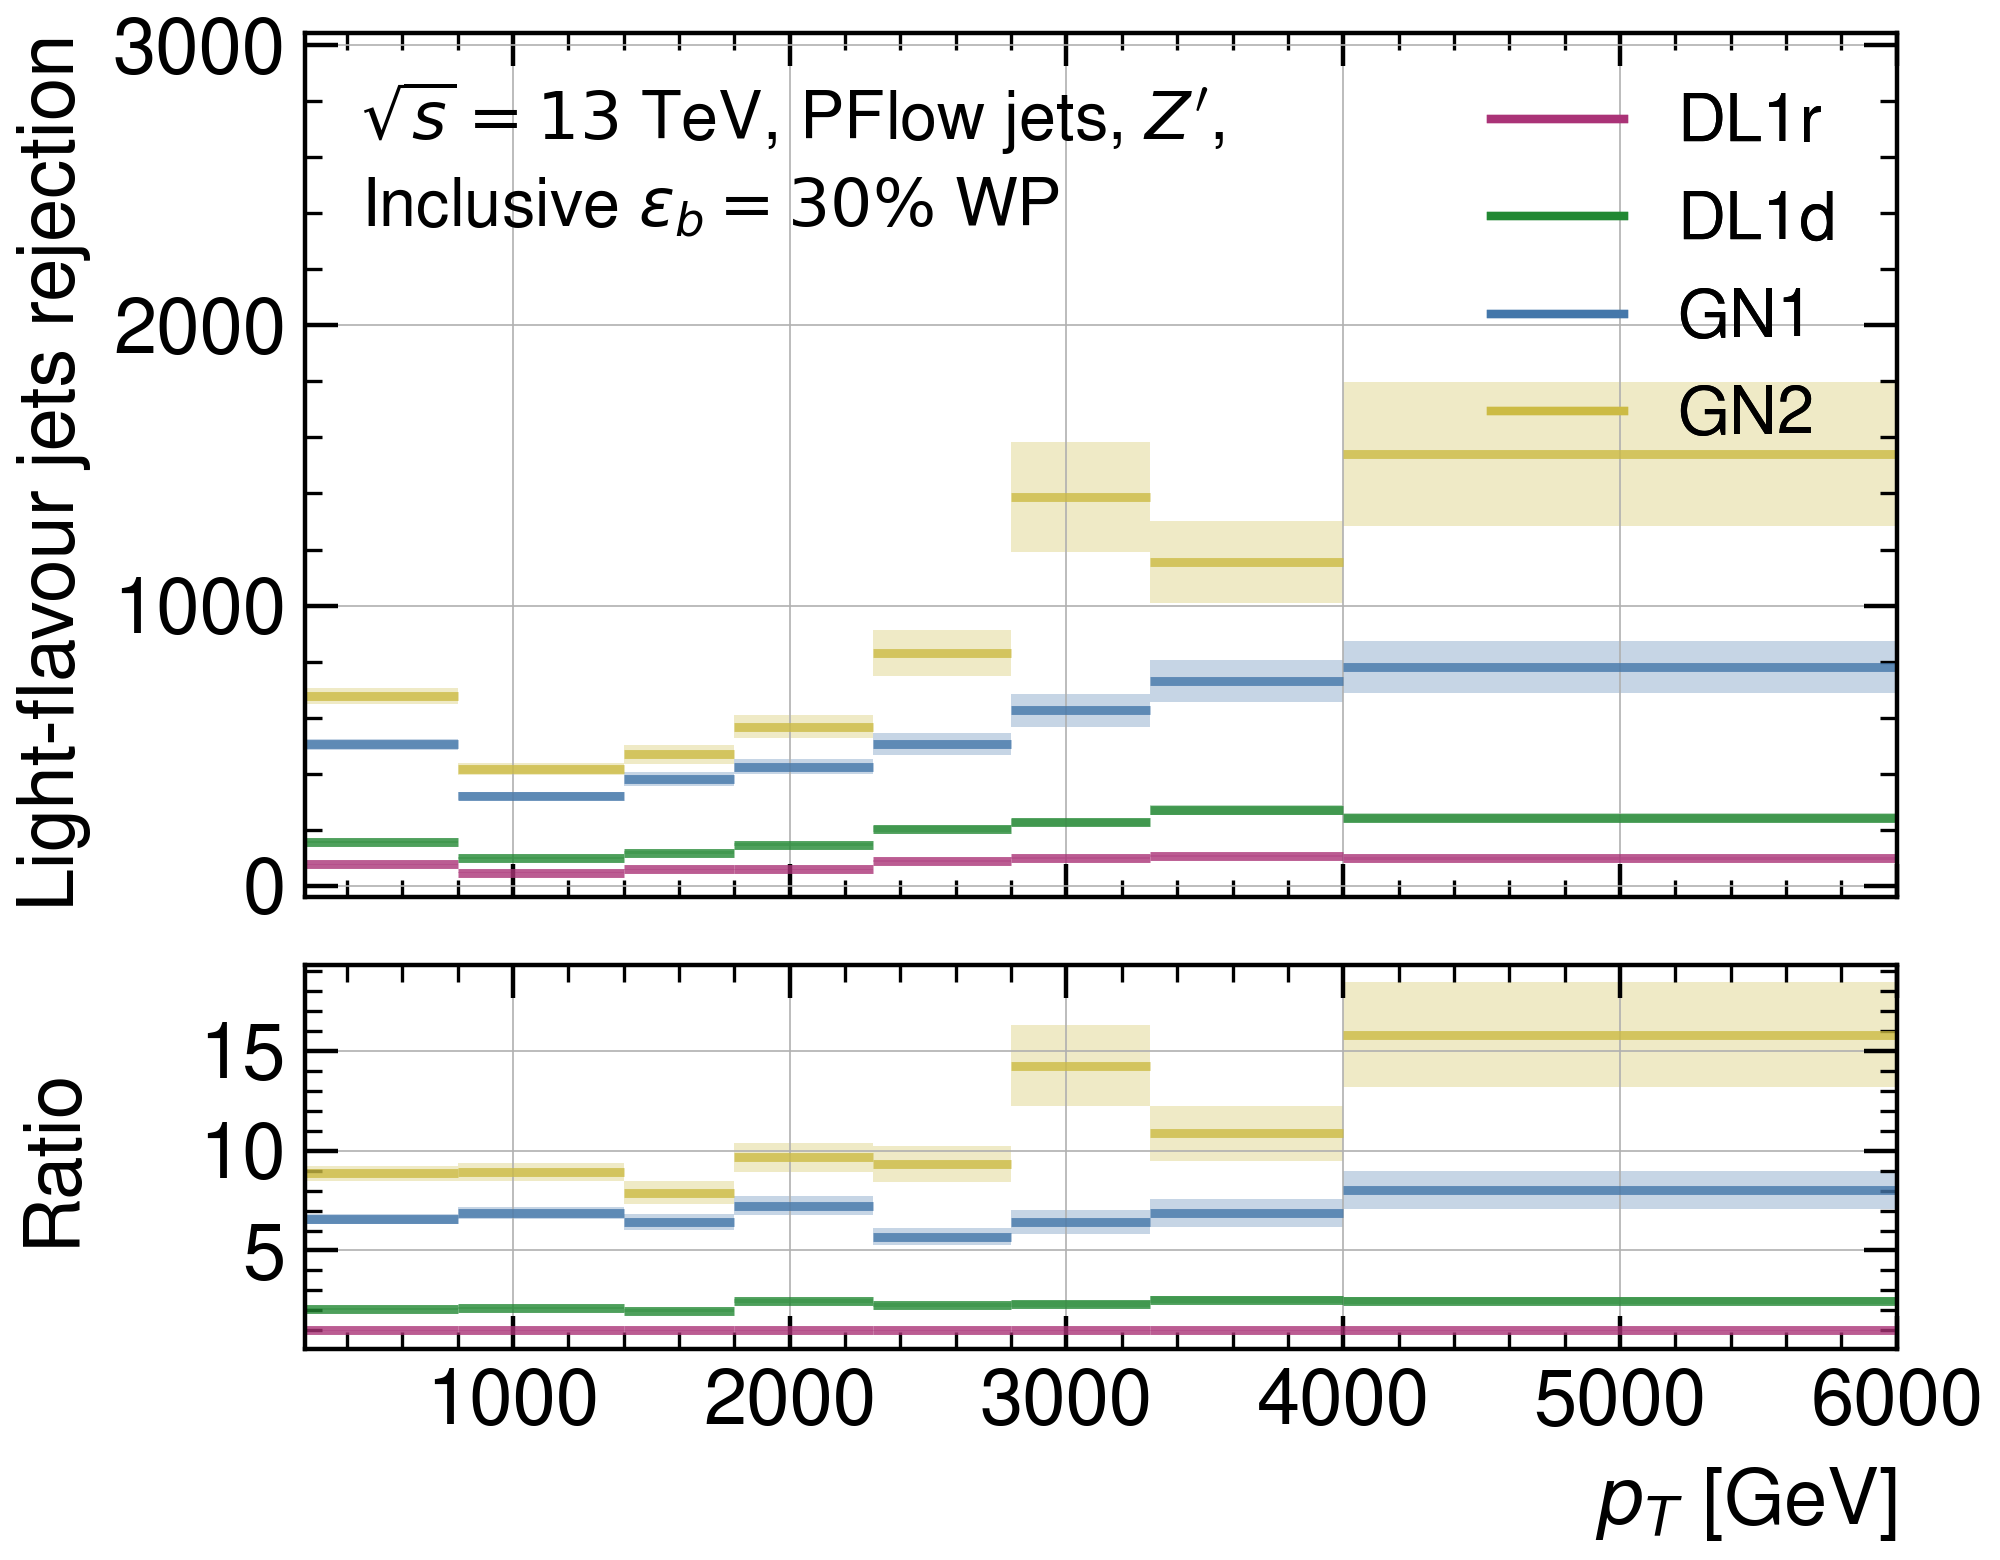
\includegraphics[width=0.48\textwidth]{Images/FTAG/GN/GN2/pt_plots/pt_zp_light_rej.png}
    \caption{Comparing the different models light-rejection as a function of jet $p_T$ for the $b$-tagging inclusive 70\% working point on the $t\bar{t}$ (left) and 30\% working point on $Z'$ (right). The flavour fraction is set at $f^b_c = 0.018$ for DL1r and DL1d, 0.05 for GN1, and 0.1 for GN2.}
    \label{apfig:GNxptb_urej}
  \end{figure} 
  
% Rej b - ctagging
\begin{figure}[h!]
    \centering
    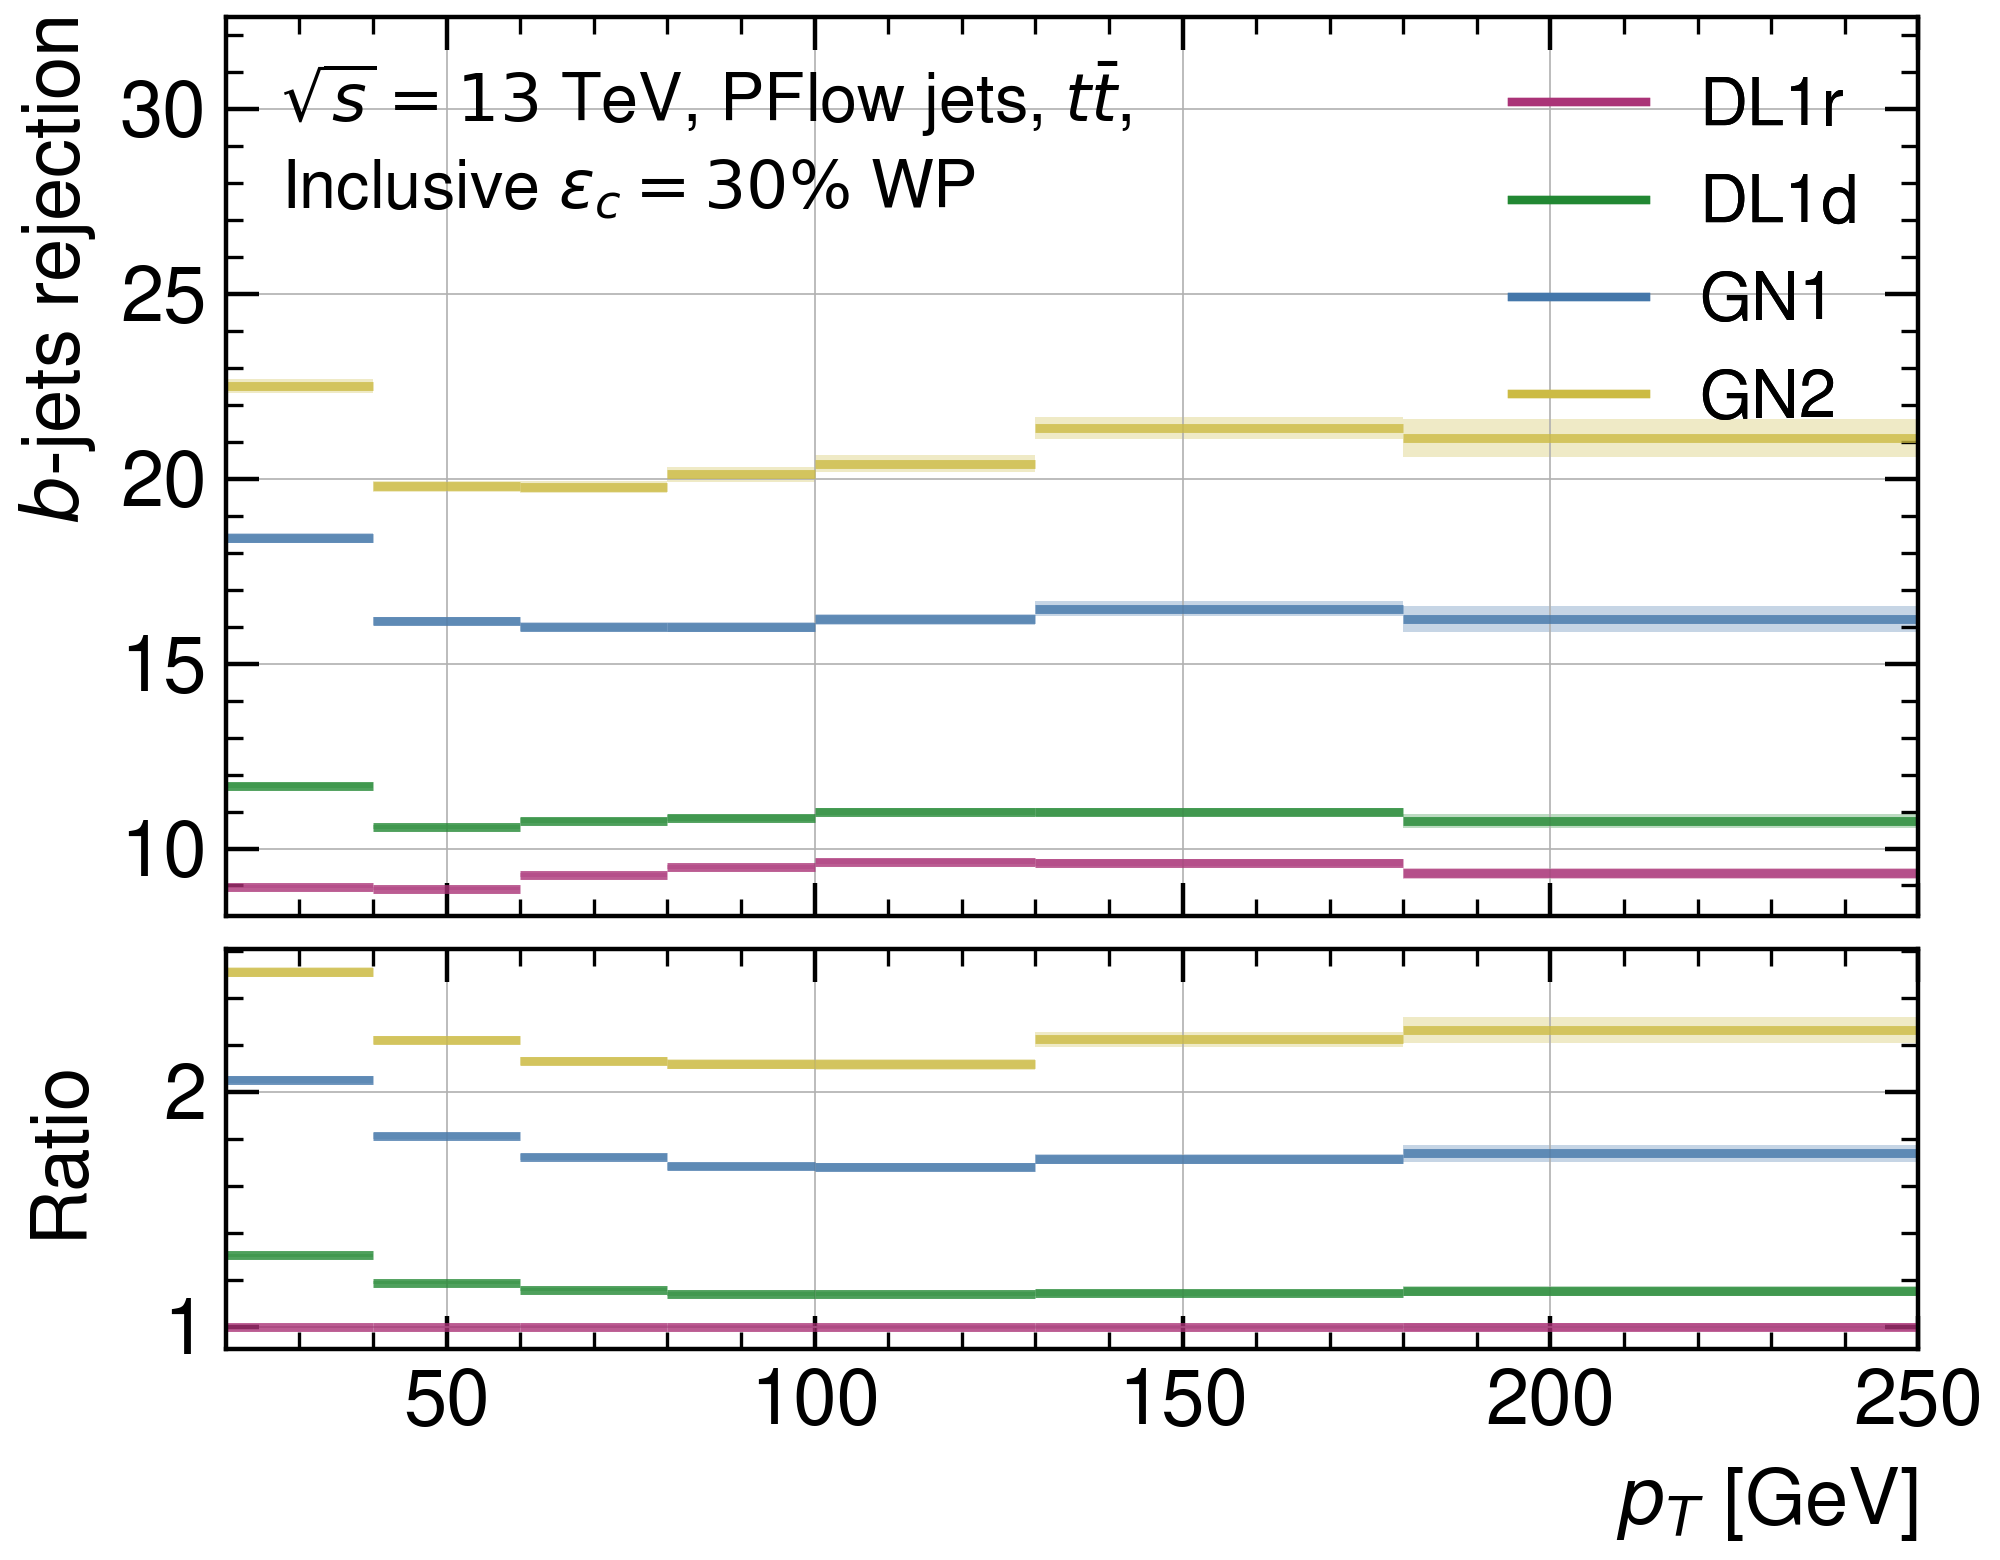
\includegraphics[width=0.48\textwidth]{Images/FTAG/GN/GN2/pt_plots/pt_ttbar_b_rej_c.png}
    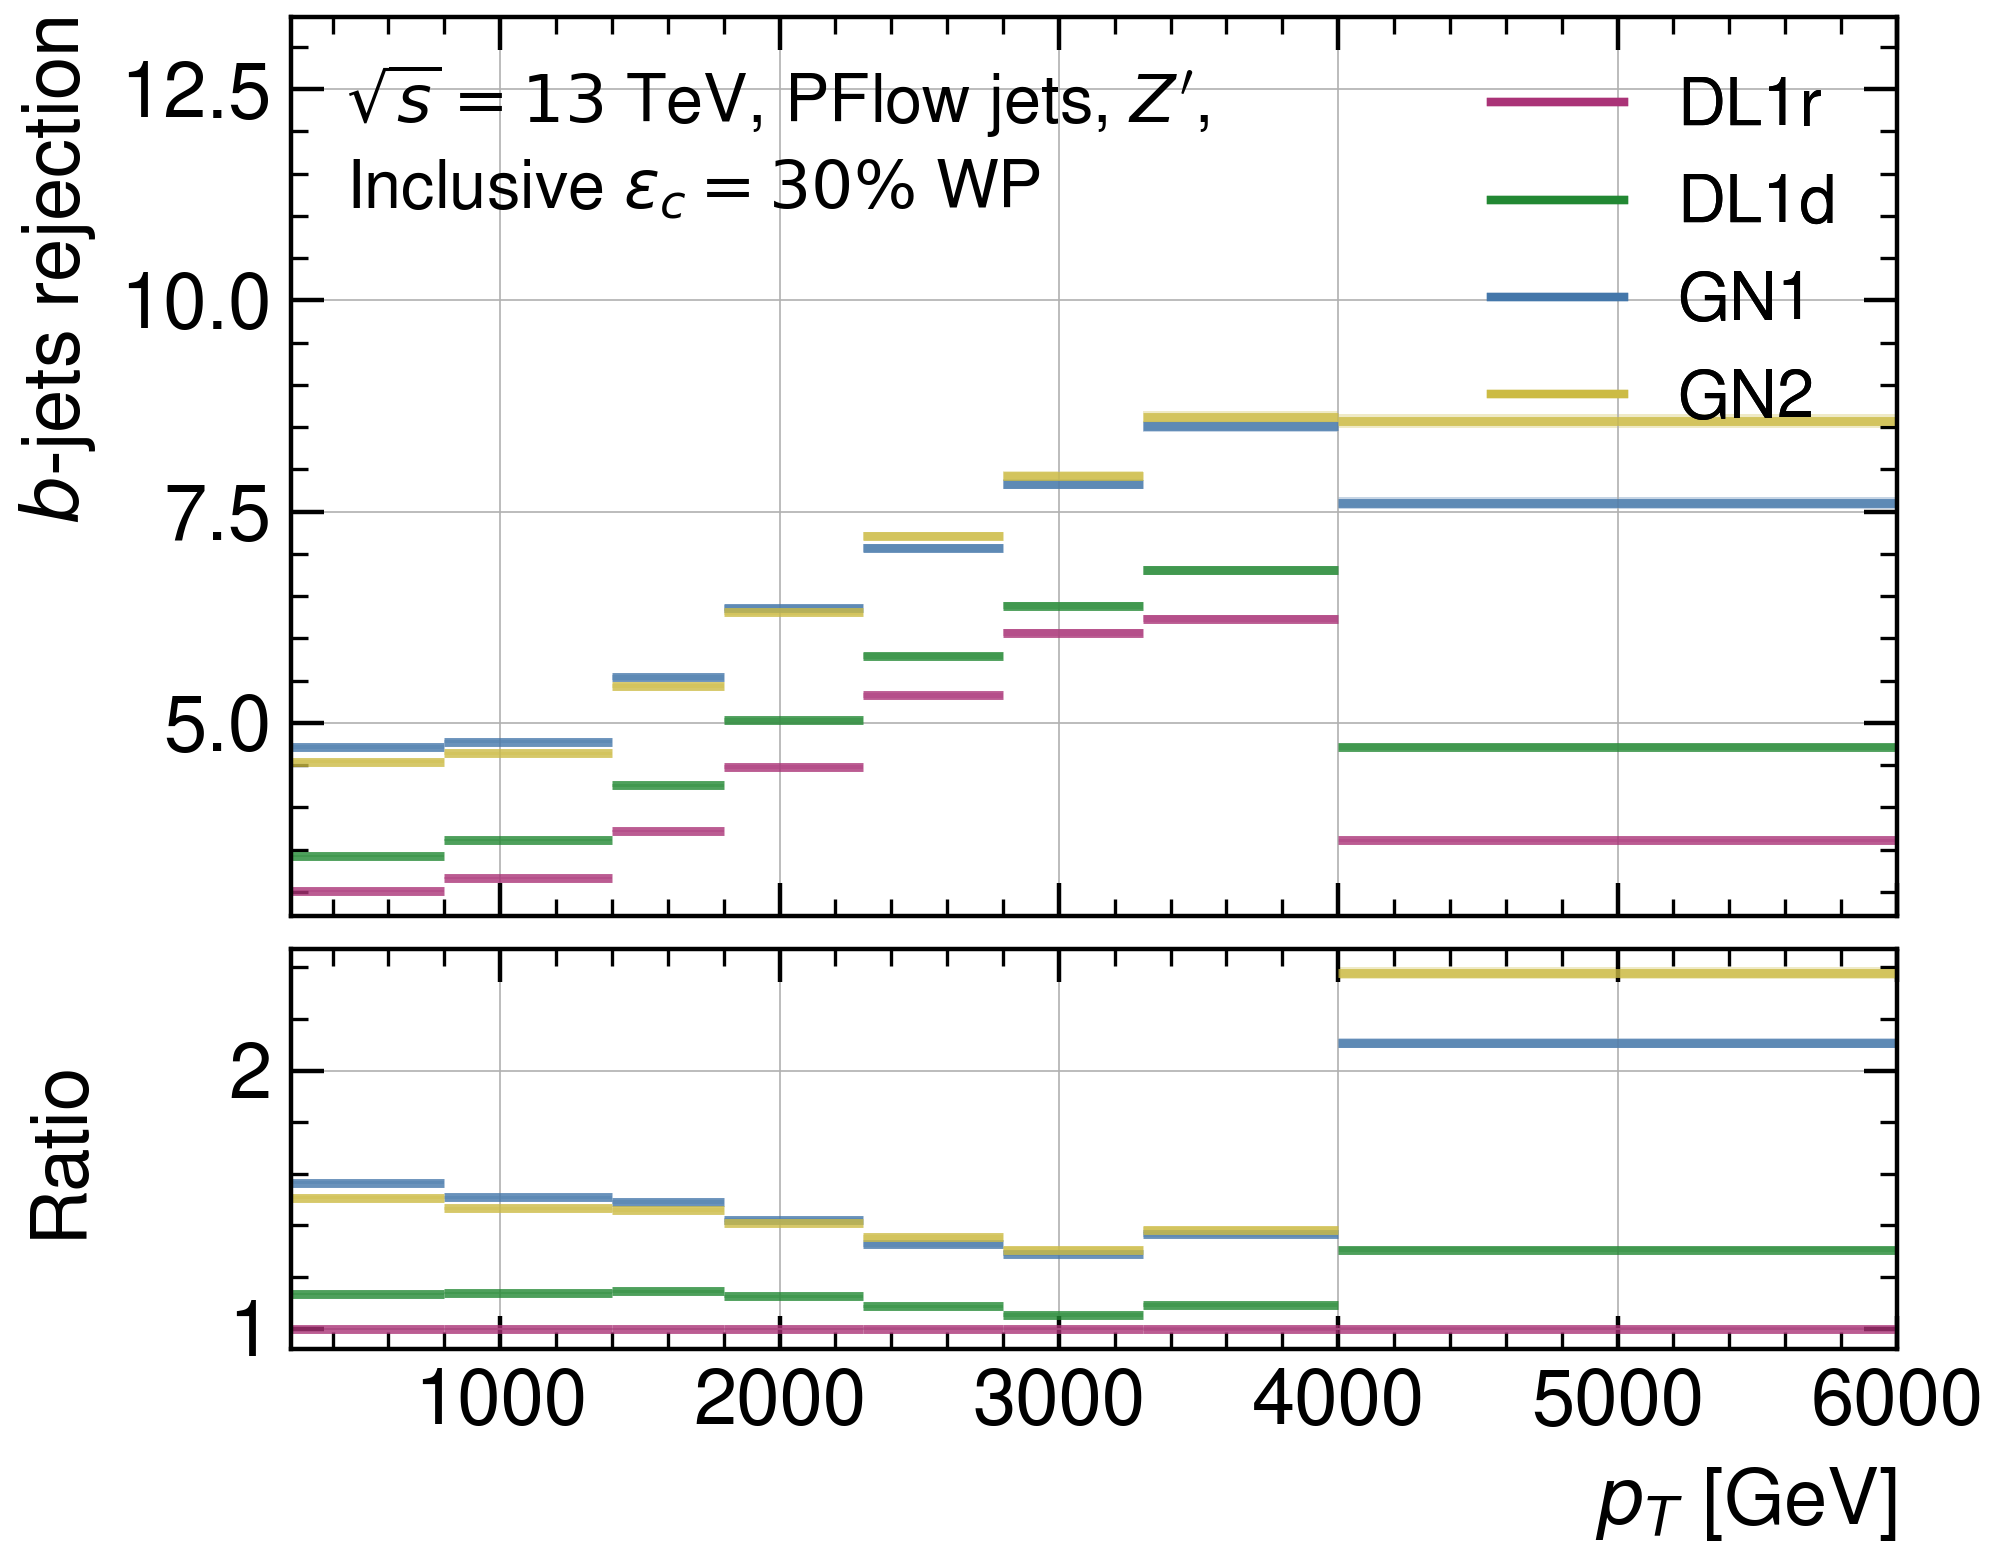
\includegraphics[width=0.48\textwidth]{Images/FTAG/GN/GN2/pt_plots/pt_zp_b_rej_c.png}
    \caption{Comparing the different models $b$-rejection as a function of jet $p_T$ for the $c$-tagging inclusive 30\% working point on the $t\bar{t}$ (left) and $Z'$ (right). The flavour fraction is set at $f^c_b = 0.2$ for all taggers.}
    \label{apfig:GNxptc_brej}
  \end{figure} 
  
  % Rej light - ctagging
  \begin{figure}[h!]
    \centering
    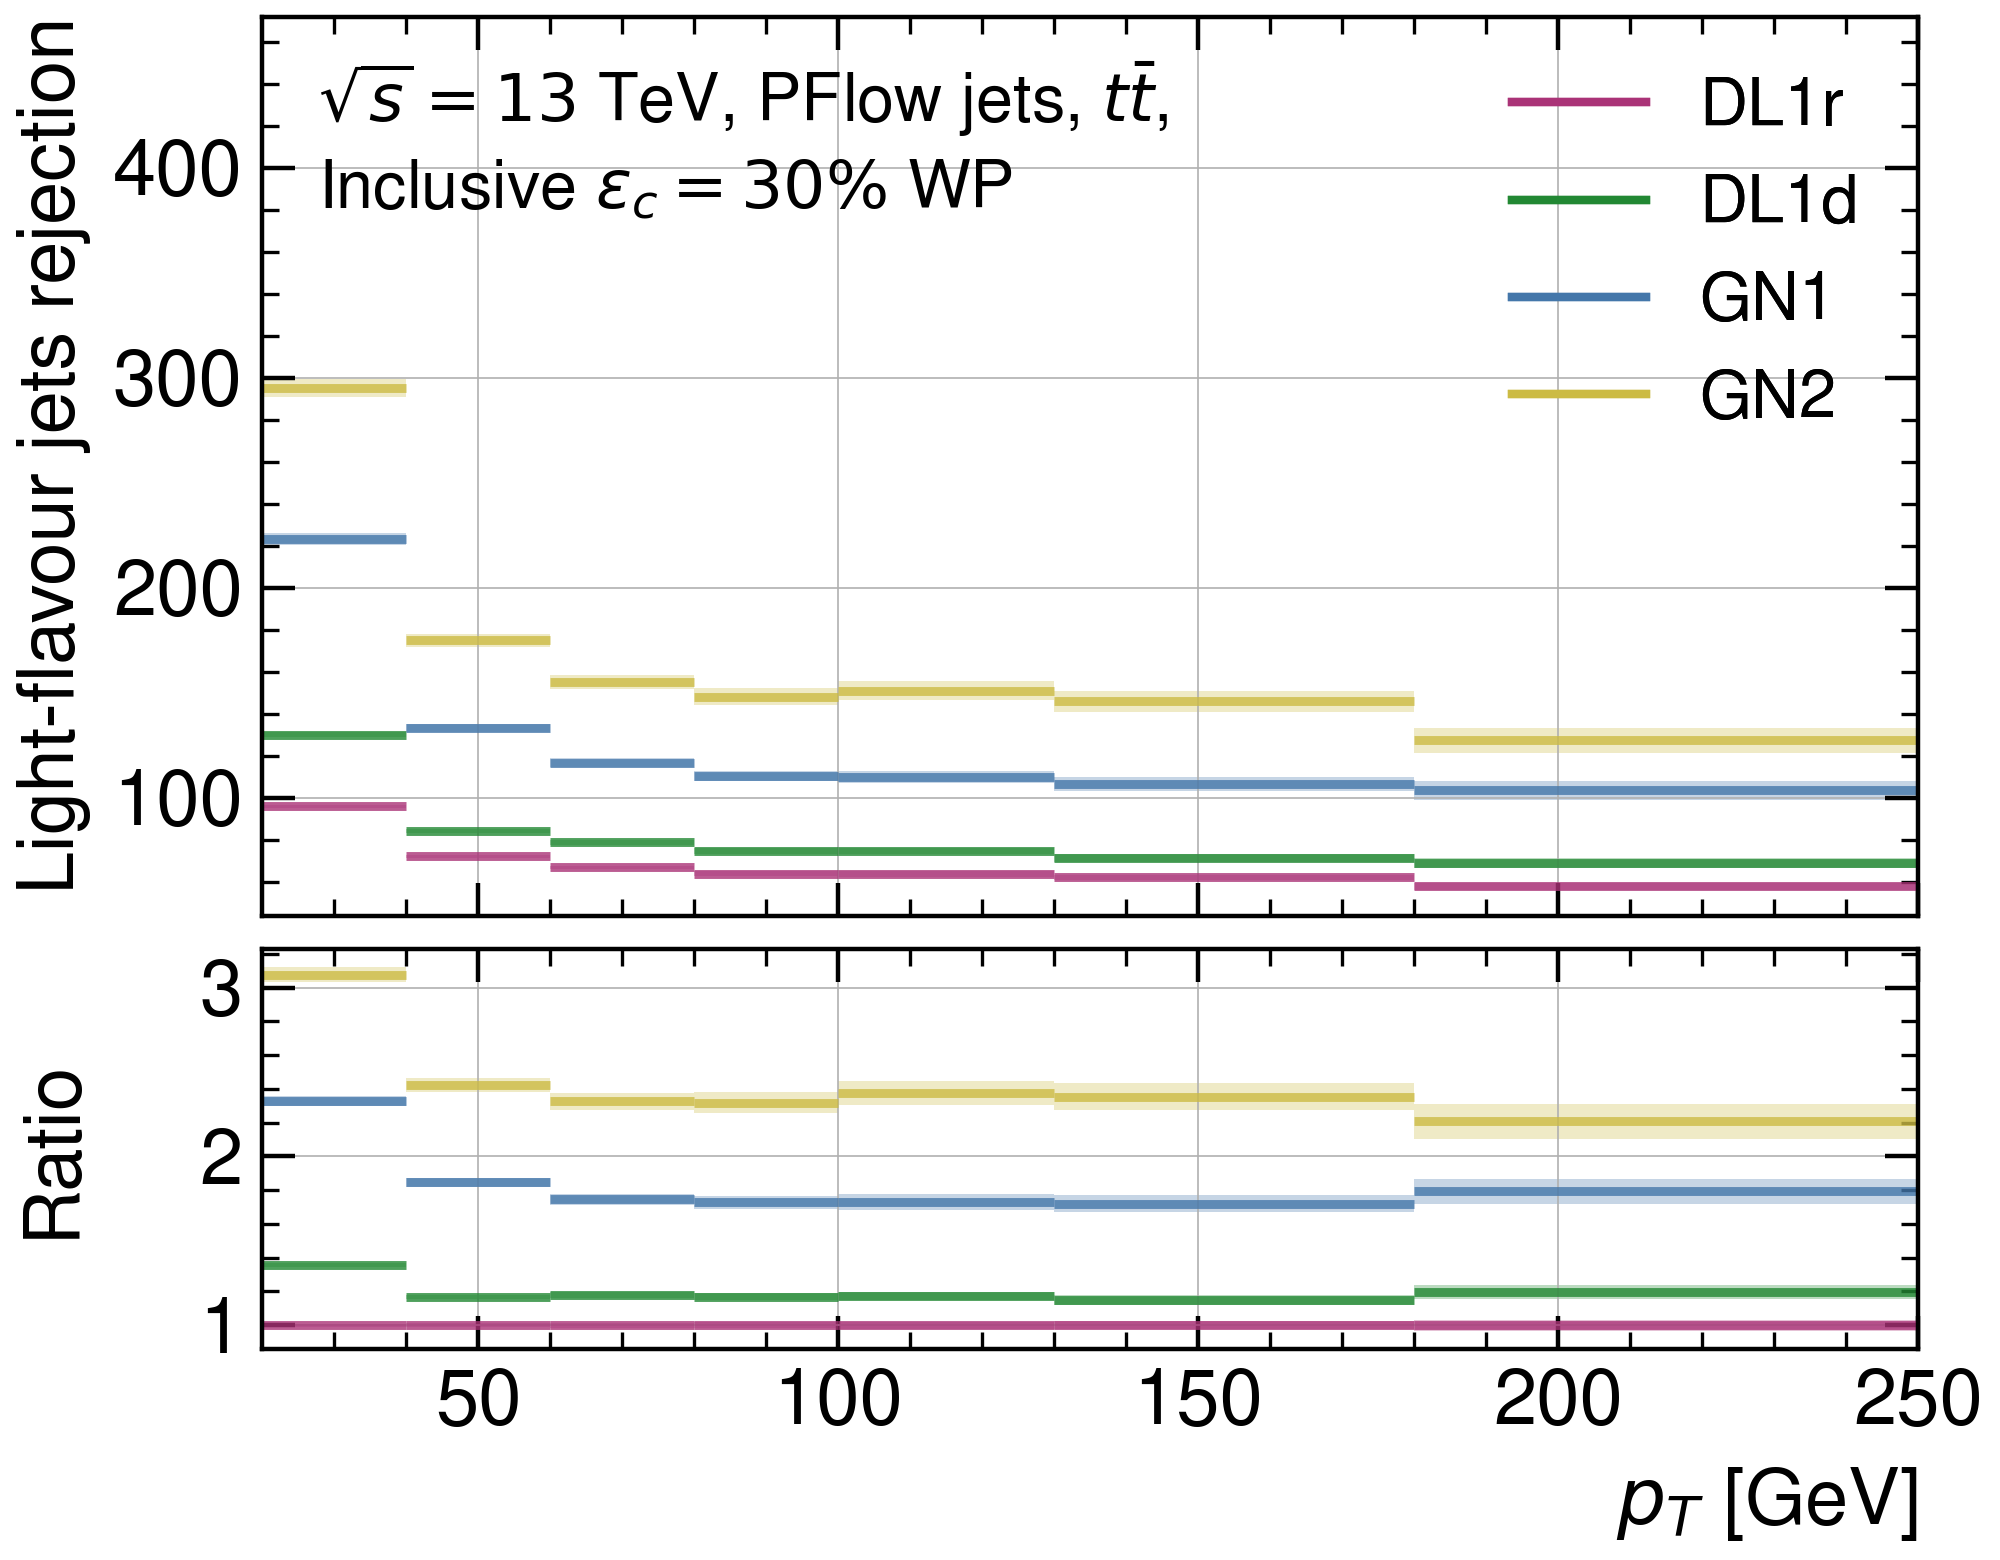
\includegraphics[width=0.48\textwidth]{Images/FTAG/GN/GN2/pt_plots/pt_ttbar_light_rej_c.png}
    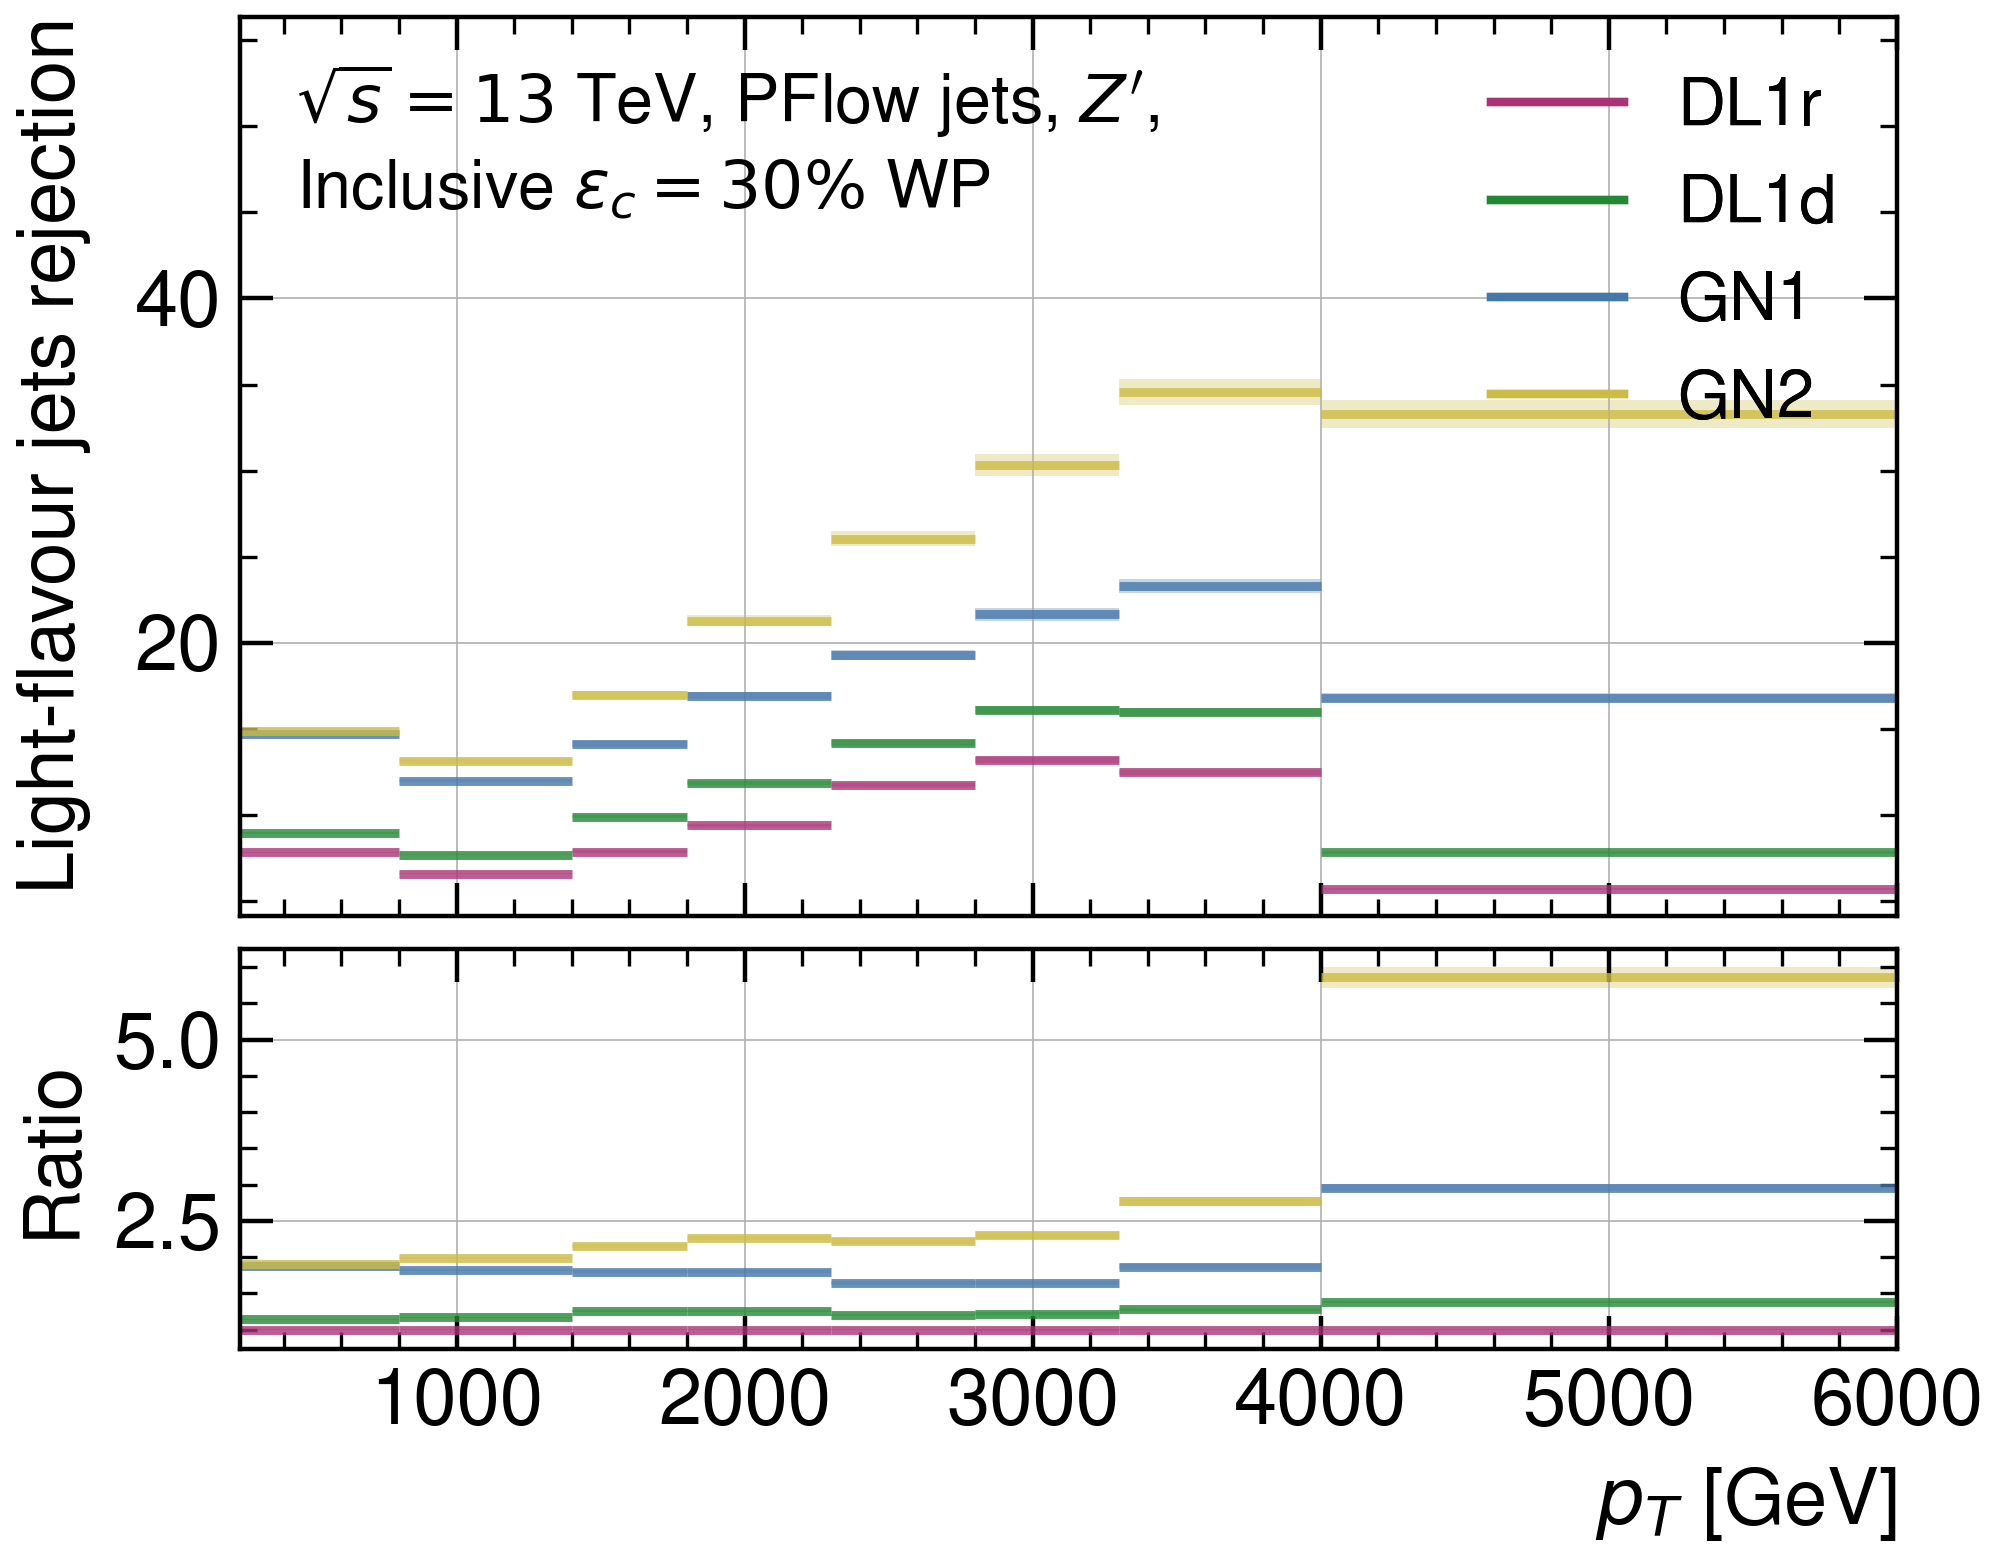
\includegraphics[width=0.48\textwidth]{Images/FTAG/GN/GN2/pt_plots/pt_zp_light_rej_c.png}
    \caption{Comparing the different models light-rejection as a function of jet $p_T$ for the $c$-tagging inclusive 30\% working point on the $t\bar{t}$ (left) and  $Z'$ (right). The flavour fraction is set at $f^c_b = 0.2$ for all taggers.}
    \label{apfig:GNxptc_urej}
  \end{figure} 